\documentclass[12pt]{report}

\usepackage{hyperref}
\usepackage{geometry}
\usepackage{amsmath}
\usepackage{enumerate}
\usepackage{mathtools}
\usepackage{amsthm}
\usepackage{amssymb}
\usepackage{caption}
\usepackage{graphicx}
\usepackage{float}
\usepackage{subfig}
\usepackage{physics}
\usepackage{bm}

\graphicspath{ {./images/} }
\geometry{margin=2cm}

\title{\textbf{Probability For the Enthusiastic Beginner \\ David Morin \\ \hfill \\ Exercise Solutions}}
\author{Stefan Stefanache}

\begin{document}
    \maketitle
    \tableofcontents
    \chapter{Combinatorics}

\section*{1.1. Assigning seats}
\addcontentsline{toc}{section}{1.1. Assigning seats}
Six girls and four boys are to be assigned to ten seats in a row, with the stipulations
that a girl sits in the third seat and a boy sits in the eighth seat. How many arrangements
are possible?

\vspace{1em}

\begin{proof}
    We compute the number of ways that the boy on the eighth seat and the girl on the third seat can be chosen:
    \[
        \binom{6}{1}\binom{4}{1} = 24
    \]

    Now, we see how many ways the other kids can be placed on the seats:
    \[
        !8 = 40,320
    \]

    Our final result is:
    \[
        24 \cdot 40,320 = 967,680
\]
\end{proof}

\section*{1.2. Number of outcomes}
\addcontentsline{toc}{section}{1.2. Number of outcomes}
One person rolls two six-sided dice, and another person flips six two-sided coins.
Which setup has the larger number of possible outcomes, assuming that the order matters?

\vspace{1em}

\begin{proof}
    The two dice rolls have $6^2 = 36$ possible outcomes, while the coin flips have $2^6 = 64$ outcomes.
\end{proof}

\section*{1.3. Subtracting the repeats}
\addcontentsline{toc}{section}{1.3. Subtracting the repeats}
\begin{enumerate}[(a)]
    \item From Eq. (1.6) we know that the number of ordered sets of three people chosen from five people
        is $5 \cdot 4 \cdot 3 = 60$. Reproduce this result by starting with the naive answer of $5^3 = 125$
        ordered sets where repetitions are allowed, and then subtracting off the number of triplets that have
        repeated people.
    \item It's actually not much more difficult to solve this problem in the general case where triplets
        are chosen from N people, instead of five. Repeat part (a) for a general N.
\end{enumerate}

\vspace{1em}

\begin{proof}
    \hfill
    \begin{enumerate}[(a)]
        \item The number of triplets that have three repeating people is obviously $5$, while the number of 
            triplets with two repetitions is given by $5 \cdot 4 \cdot 2 + 5 \cdot 1 \cdot 4 = 60$. 
            Therefore, the number of ordered sets of three people chosen from five people is $125 - 60 = 65$.

        \item The number of triplets that have three repeating people will be $N$, while the number of triplets
            that have two repeating people will be $N(N - 1) \cdot 2 + N(N - 1) = 3N(N-1)$. As a result,
            the number of ordered sets of three people chosen from five people is given by
            $N^3 - 3N(N - 1) - N = N^3 - 3N^2 + 2N$.
    \end{enumerate}
\end{proof}

\section*{1.4. Subtracting the repeats, again}
\addcontentsline{toc}{section}{1.4. Subtracting the repeats, again}
Repeat the task of Problem 1.3(a), but now in the case where you pick quadruplets (instead of triplets)
from five people.

\vspace{1em}

\begin{proof}
    The number of ordered sets of 4 people chosen from five people is $5 \cdot 4 \cdot 3 \cdot 2 = 120$.

    To find the number of repeating quadruplets, we split them into 3 categories:
    \begin{enumerate}
        \item \textbf{4 repeating people} The repeating person can be chosen in 5 ways and there is only one way
            to order (AAAAA), so there are 5 such quadruples.

        \item \textbf{3 repeating people} The repeating person can be chosen in 5 ways, and then the 
            non-repeating person in 4 ways, thus the number of unorderd quadruples is given 
            by $4 \cdot 5 = 20$. Since there are 4 (AAAB, AABA, ABAA, BAAA) ways to choose the 
            order, we get $4 \cdot 20 = 80$ ordered quadruples.

        \item \textbf{2 repeating people} The repeating person can be chosen in 5 ways, and the other 2 people
            can be chosen in $\binom{4}{2} = 6$ ways. Therefore, we have $5 \cdot 30 = 50$ unordered quadruples.
            The sets can be ordered in 12 ways, so we have $30 \cdot 12 = 360$ orderd quadruples with 2 
            repeating people.

        \item \textbf{2 groups of repeating people} The repeated persons can be chosen in $\binom{5}{2} = 10$ 
            ways and can be ordered in 6 modes (AABB, ABAB, ABBA, BBAA, BABA, BAAB), therefore the number
            of such sorted quadruples is 60.

            Therefore, the number of ordered sets of four people from five people is 
            \[
                5^4 - 5 - 80 - 360 - 60 = 120
            \] 
    \end{enumerate}
\end{proof}

\vspace{1em}

\section*{1.6. Many ways to count}
\addcontentsline{toc}{section}{1.6. Many ways to count}
How many different orderings are there of the six letters: A, A, A, B, B, C? \\
How many different ways can you think of to answer this question?

\vspace{1em}

\begin{proof}
    We analyze the possible orderings of the letters. The positions of the 3 A letters can be chosen 
    in $\binom{6}{3} = 20$ ways, and then the positions of the two B letters can be chosen in
    $\binom{3}{2} = 3$ modes. Since the C letter has the last position, we find that the number of possible
    orderings is now $20 \cdot 3 = 60$.

    The same method can be applied for any ordering of letter-position assignments (e.g. we choose the 
    possible positions of B and then of A and C). We'll get different formulas, but the result will be the
    same. There are $3 \cdot 2 = 6$ such ways of computing the number of possible orderings.
\end{proof}

\section*{1.7. Committees with a president}
\addcontentsline{toc}{section}{1.7. Committees with a president}
Two students are given the following problem: From $N$ people, how many ways are there to choose a committee
of $n$ people, with one person chosen as the president? One student gives an answer of $n\binom{N}{n}$, while
the other student gives an answer of $N\binom{N-1}{n-1}$.

\begin{enumerate}[(a)]
    \item By writing out the binomial coefficients, show that the two answers are equal.
    \item Explain the (valid) reasoning that lead to these two (correct) answers.
\end{enumerate}

\vspace{1em}

\begin{proof}
    \hfill
    \begin{enumerate}[(a)]
        \item We simply rewrite the expressions to obtain the equality:
        \[
            n\binom{N}{n} = n\frac{N!}{n!(N-n)!} = \frac{N!}{(n-1)!(N-n)!} = N\frac{(N-1)!}{(n-1)!(N-n)!}
                          = N\binom{N-1}{n-1}
        \]
        \item The president can be chosen in $N$ ways and then the rest of the group can be chosen in 
            $\binom{N-1}{n-1}$ modes, giving us $N\binom{N-1}{n-1}$ ways to form the committee.

            Without thinking about the president, the committee can be chosen in $\binom{N}{n}$ ways. In 
            such a committee any of the $n$ persons can be chosen as the president. Therefore, we have 
            $n\binom{N}{n}$ ways to form the committee.
    \end{enumerate}
\end{proof}

\section*{1.8. Multinomial coefficients}
\addcontentsline{toc}{section}{1.8. Multinomial coefficients}
\begin{enumerate}[(a)]
    \item A group of ten people are divided into three committees. Three people are on committee
        A, two are on committee B, and five are on committee C. How many different ways are there 
        to divide up the people?

    \item
        A group of N people are divided into k committees. $n_1$ people are on committee 1, $n_2$
        people are on committee 2, \dots, and $n_k$ people are on committee $k$, with 
        $n_1 + n_2 + \dots + n_k = N$. How many different ways are there to divide up the people?
\end{enumerate}

\vspace{1em}

\begin{proof}
    \hfill
    \begin{enumerate}[(a)]
        \item The people on committee A can be chosen in $\binom{10}{3} = 120$ ways and then the people on
            committee B can be chosen in $\binom{7}{2} = 21$ ways. The remaining people will be on the C
            committee. As a result, the group of ten people can be divided in $120 \cdot 21 = 2,520$ ways.
        
        \item We assign people to committees like in the previous example. The 1st committee's members
            can be chosen in $\binom{N}{n_1}$ modes, the 2nd committee's composition can be chosen in 
            $\binom{N - n_1}{N_2}$ ways, and so on. We observe (and can prove using induction), that the
            number of ways the i-th ($2 \leq i < k$) committee can be assembled is given by the expression:
            \[
                M_i = \binom{N - n_1 - \ldots - n_{i - 1}}{n_i}
            \]
            Therefore, the number of ways the group of people can be divided is given by:
            \begin{align*}
                M = \binom{N}{n_1} \prod_{i = 2}^{k}M_i 
                    =& \binom{N}{n_1} \binom{N - n_1}{n_2} \ldots \binom{N - n_1 - \ldots - n_{k - 1}}{n_k} \\
                    =& \frac{N!}{n_1! (N - n_1)!} \cdot \frac{(N - n_1)!}{n_2! (N - n_1 - n_2)!} \cdot \ldots 
                    \cdot \frac{(N - n_1 - \ldots - n_{k - 1})!}{n_3! (N - n_1 - \ldots - n_{k - 1} - n_k)!} \\
                    =& \frac{N!}{n_1!n_2! \ldots n_k!}
            \end{align*}
    \end{enumerate}
\end{proof}

\section*{1.9. One heart and one 7}
\addcontentsline{toc}{section}{1.9. One heart and one 7}
How many different five-card poker hands contain exactly one heart and exactly one 7? (If the hand
contains the 7 of hearts, then this one card satisfies both requirements.)

\vspace{1em}

\begin{proof}
    There are $52 - 13 - 4 + 1 = 36$ cards that are neither a heart nor a 7. We consider two cases:
    \begin{enumerate}[(i)]
        \item \textbf{The 7 of hearts is in the hand}, so the other 4 cards in the hand
            can be any that are neither a heart nor a 7. As a result, we have 
            $\binom{36}{4}= 58,905$ such hands.

        \item \textbf{The 7 of hearts is not in the hand.} There are 12 cards that are hearts and 
            not a 7 and 3 cards that are 7 but not a heart. We choose one of each and the rest of 
            the cards can be any that are neither a heart nor a 7. Hence, we get
            $12 \cdot 3 \binom{36}{3} = 257,040$ such hands.
    \end{enumerate}
    In conclusion, there are $286,110 + 257,040 = 315,945$ five-card hands that contain exactly
    one heart and exactly one 7.
\end{proof}


\section*{1.14. Yahtzee}
\addcontentsline{toc}{section}{1.14. Yahtzee}
In the game of Yahtzee, five dice are rolled in a group, with the order not mattering.

\begin{enumerate}[(a)]
    \item Using Eq. (1.16), how many unordered rolls (sets) are possible?

    \item In the spirit of the examples at the beginning of Section 1.7. reproduce the
        result in part (a) by determining how many unordered rolls there are
        of each general type (for example, three of one number and two of another, etc.)

    \item In the spirit of the example at the end of Section 1.7., show that the total
        number of \emph{ordered} Yahtzee rolls is $6^5 = 7776$.
\end{enumerate}

\vspace{1em}

\begin{proof}
    \hfill
    \begin{enumerate}[(a)]
        \item The number of unordered rolls is given by 
            \[
                \binom{5 + (6 - 1)}{6 - 1} = \binom{10}{5} = 252
            \] 

        \item We split the rolls in 7 types:
            \begin{enumerate}[(1)]
                \item All five rolls are the same (e.g. 66666). There are 6 sets of this type.

                \item Four rolls have the same value and the other roll has another value (e.g. 66665).
                    There are $6 \cdot 5 = 30$ sets of this type.
                
                \item Three rolls have the same value and the other two rolls have other (different 2 by 2)
                    values (e.g. 66654). There are  $6 \binom{5}{2} = 6 \cdot 10 = 60$ sets of this type.

                \item Three rolls have the same value and the other two rolls have both another (same) value 
                    (e.g. 66655). There are $6 \cdot 5 = 30$ sets of this type.

                \item Two rolls have the same value and the other three rolls have different (2 by 2) values
                    (e.g. 66654). There are $6 \binom{5}{2} = 60$ such sets.

                \item Two rolls have the same value, two rolls have another (same value) and the 
                    remaining roll has another different value (e.g. 66554). 
                    There are $6 \binom{5}{2} = 60$ such sets of rolls.

                \item Each roll has a different value. (e.g. 65432). There are $\binom{6}{5} = 6$ such sets.
            \end{enumerate}

        By summing all the types, we get that the number of unordered rolls is 
        \[
            6 + 30 + 60 + 30 + 60 + 60 + 6 = 252
        \] 

    \item We want to see in how many ways can the 5 roll types be ordered:
        \begin{enumerate}[(1)]
            \item All rolls are the same, so the set can be ordered in one way. The number of 
                ordered sets with the same 5 rolls is 6.

            \item Four rolls have the same value and the other roll has another value.
                The set can be ordered in 5 ways (we consider the different roll on each
                possible position). Therefore, there are $5 \cdot 30 = 150$ ordered sets of this type.

            \item Three rolls have the same value and the other two have other (different 2 by 2) values.
                The positions of the repeated values can be chosen in $\binom{5}{3} = 10$ and then there 
                are two ways to order the other values, so there are $10 \cdot 2 = 20$ ways to order the set.
                As a result, there are $20 \cdot 60 = 1200$ ordered sets of this type.

            \item Three rolls have the same value and the other two rolls have both another (same) value.
                There are $\binom{5}{3} = 10$ ways the sets can be ordered, so we get $10 \cdot 30 = 300$
                such ordered sets.

            \item Two rolls have the same value and the other three have other (different 2 by 2) values.
                As before, we find that the set of values can be ordered in 
                $\binom{5}{2} \cdot 3 \cdot 2 = 60$ ways.
                Hence, there are $60 \cdot 60 = 3600$ such ordered sets.

            \item Two rolls have the same value, two rolls have another (same value) and the 
                remining roll has another differente value. There are 
                $\binom{5}{2}\binom{3}{2} = 10 \cdot 3 = 30$ ways to order this set, so we get 
                $30 \cdot 60 = 1800$ such ordered sets.

            \item All rolls have different values. The sets can be ordered in $5! = 120$ ways. As a result,
                there are $120 \cdot 6 = 720$ such ordered sets.
        \end{enumerate}

        In conclusion, we get that the number of $\emph{ordered}$ sets of Yahtzee rolls is:
        \[
            6 + 150 + 1200 + 300 + 3600 + 1800 + 720 = 7776 = 6^5
        \] 
    \end{enumerate}
\end{proof}

\section*{1.16. Pascal sum 2}
\addcontentsline{toc}{section}{1.16. Pascal sum 2}
At the end of Section 1.8.3, we demonstrated the relation 
$\binom{n}{k} = \binom{n - 1}{k - 1} + \binom{n - 1}{k}$
by using the argument involving committees. Repeat this reasoning,
but now in terms of:
\begin{enumerate}[(a)]
    \item coin flips,
    \item the $(a + b)^n$ binomial expansion.
\end{enumerate}

\vspace{1em}

\begin{proof}
    \hfill
    \begin{enumerate}[(a)]
        \item The number of ways we can get $k$ tails from $n$ coin flips is given by 
            $\binom{n}{k}$. If we single out the first flip, we get two cases:
            \begin{enumerate}[(1)]
                \item The flip was heads, so the number of ways to get tails $k$ times
                    from the rest $n - 1$ of the flips is $\binom{n - 1}{k}$

                \item The flip was tails, so the number of ways to get the remaining 
                    $k - 1$ tails flips from the other $n - 1$ rolls is given by $\binom{n - 1}{k - 1}$
            \end{enumerate}

        Therefore, the number of ways we get $k$ tails from $n$ coin flips can be split into the above
        two cases, so:
        \[
            \binom{n}{k} = \binom{n - 1}{k} + \binom{n - 1}{k - 1}
        \] 

    \item The coefficient of the term $a^{n - k}b^k$ from the expansion of $(a + b)^n$ is given by 
        $\binom{n}{k}$. If we single out the first $(a + b)$ factor, we have two possible situations:
        \begin{enumerate}
            \item The factor was used in getting a power of $b$ in $a^{n - k}b^k$, so there are 
                $\binom{n - 1}{k - 1}$ factors to use for the other $k - 1$ powers of $b$ and the $n - k$ 
                powers of $a$, since 
                $\binom{n - 1}{n - k} = \binom{n - 1}{k - 1}$.

            \item The factor wasn't used in getting a power of $b$ in $a^{n - k}b^k$, so there are 
                $\binom{n - 1}{k}$ factors to use for the other $k$ b powers and the other $n - k - 1$ 
                powers of a, since $\binom{n - 1}{n - k - 1} = \binom{n - 1}{k}$.
        \end{enumerate}

    Therefore, the coefficient of $a^{n-k}b^k$ is given by:
    \[
        \binom{n}{k} = \binom{n - 1}{k} + \binom{n - 1}{k - 1}
    \] 
    \end{enumerate}
\end{proof}

\section*{1.17. Pascal diagonal sum}
\addcontentsline{toc}{section}{1.17. Pascal diagonal sum}
\begin{enumerate}[(a)]
    \item If we pick an unordered committee of three people from five people (A, B, C, D, E),
        we can list the $\binom{5}{3} = 10$ possibilities as shown in Table 1.19.
        We have grouped them according to which letter comes first. (The order of letters
        doesn't matter, so we've written each triplet in increasing alphabetical order.)
        The columns in the table tell us that we can think of $10$ as equaling $6 + 3+ 1$.
        Explain why it makes sense to write this sum as  $\binom{4}{2} + \binom{3}{2} + \binom{2}{2}$.

        \begin{table}[h]
            \centering
            \begin{tabular}{ccc}
                A B C & & \\ 
                A B D & & \\
                A B E & & \\
                A C D & B C D & \\
                A C E & B C E & \\
                A D E & B D E & C D E \\
            \end{tabular}
            \caption*{\textbf{Table 1.19:} Unordered triplets chosen from five people.}
        \end{table}

    \item You can also see from Table 1.15 and 1.16 that, for example 
        $\binom{6}{3} = \binom{5}{2} + \binom{4}{2} + \binom{3}{2} + \binom{2}{2}$.
    More generally,
    \begin{equation*}\tag{1.29}
        \binom{n}{k} = \binom{n - 1}{k - 1} + \binom{n - 2}{k - 2} + \binom{n - 3}{k - 3} + \ldots + 
                        \binom{k}{k - 1} + \binom{k - 1}{k - 1}
    \end{equation*}

    In words: A given number (for example, $\binom{6}{3}$) in Pascal's triangle equals the sum
    of the numbers in the diagonal string that starts with the number that is above and to the 
    left of the given number ($\binom{5}{2}$ in this case) and then proceeds upward to the right.
    So the string contains $\binom{5}{2}, \binom{4}{2}, \binom{3}{2}$ and $\binom{2}{2}$
    in this case.

    Prove Eq.(1.29) by making repeated use of Eq.(1.22), which says that each number in Pascal's
    triangle is the sum of the two numbers abot it (or just the "1" above it, if it occurs at the end 
    of a line).
\end{enumerate}

\begin{proof}
    \hfill
    \begin{enumerate}[(a)]
        \item We split the committees into 4 categories:
            \begin{enumerate}[(1)]
                \item The set contains A, so there are $\binom{4}{2} = 6$ such sets.
                \item The set contains B and doesn't contain A, so there are $\binom{3}{2} = 3$ sets.
                \item The set contains C and doesn't contain A or B, so there is $\binom{2}{2} = 1$
                \item The set doesn't contain A, B or C. There are obviously no such sets, as we
                    need 3 elements.
           \end{enumerate}

        Since the reunion of those sets contains all the possible unordered committees of 3 members,
        we obtain that:
        \[
            \binom{4}{2} + \binom{3}{2} + \binom{2}{2} = 6 + 3 + 1 = 10 = \binom{5}{3}
        \] 
        
        \item We prove using induction that:
        \begin{equation*}\tag{1.29}
            \binom{n}{k} = \binom{n - 1}{k - 1} + \binom{n - 2}{k - 2} + \ldots + 
                            \binom{k}{k - 1} + \binom{k - 1}{k - 1}
                            = \sum_{i = k}^{n} \binom{i - 1}{k - 1}, \forall k \in \mathbb{N^*}, k \leq n
        \end{equation*}
        for all $n \in \mathbb{N}, n \geq 2$.

        The base case is obviously valid, since
        \begin{align*}
            \binom{2}{1} &= \binom{1}{0} + \binom{0}{0} = 1 + 1 = 2 \\
            \binom{2}{2} &= \binom{1}{1} + \binom{0}{1} = 1 + 0 = 1
        \end{align*}

        We assume that the relation holds for a fixed $m \in \mathbb{N}, m \geq 2$, so we have:
        \[
            \binom{m}{k} = \sum_{i = k}^{m}\binom{i - 1}{k - 1}, \forall k \in \mathbb{N^*}, k \leq n
        \]

        Using (1.22), we obtain that: 
        \[
            \binom{m + 1}{k} = \binom{m}{k} + \binom{m}{k - 1} 
                             = \sum_{i = k}^{m}\binom{i - 1}{k - 1} + \binom{m}{k - 1} 
                             = \sum_{i = k}^{m + 1}\binom{i - 1}{k - 1} 
        \] 

        Since (1.22) holds true for the base case and the $m$ case implies the validity of the $m + 1$ case,
        we proved using induction that (1.29) holds for all $n \in \mathbb{N}, n \geq 2$.
    \end{enumerate}
\end{proof}

    \chapter{Probability}

\section*{2.2. Rules for three events}
\addcontentsline{toc}{section}{2.2. Rules for three events}
\begin{enumerate}[(a)]
    \item Consider three events, $A$, $B$, and $C$. 
        If they are all independent of each other,
        show that
        \begin{equation*}\tag{2.76}
            P(A \text{ and } B \text{ and } C) = P(A) \cdot P(B) \cdot P(C) 
        \end{equation*}

    \item If they are (possibly) dependent, show that 
        \begin{equation*}\tag{2.77}
            P(A \text{ and } B \text{ and } C) = P(A) \cdot P(B | A) \cdot P(C | A \text{ and } B) 
        \end{equation*}

    \item If they are all mutually exclusive, show that
        \begin{equation*}\tag{2.78}
            P(A \text{ or } B \text{ or } C) = P(A) + P(B) + P(C)
        \end{equation*}

    \item If they are (possibly) nonexclusive, show that
        \begin{align*}\tag{2.79}
            P(A \text{ or } B \text{ or } C) =& P(A) + P(B) + P(C) \\
                                          &- P(A \text{ and } B) - P(A \text{ and } C) - P(B \text{ and } C) \\
                                          &+ P(A \text{ and } B \text{ and } C)
        .\end{align*}
\end{enumerate}

\begin{proof}
    \hfill
    \begin{enumerate}[(a)]
        \item Using (2.9) we find that:
            \[
                P(A \text{ and } B \text{ and } C) = P(A) \cdot P(B \text{ and } C | A) 
                = P(A) \cdot P(B | A) \cdot P(C | A \text{ and } B)
            .\] 
            Because the events are independent, $P(B | A) = P(B)$ and $P(C | A \text { and } B) = P(C)$, so
            \begin{equation*}\tag{2.76}
                P(A \text{ and } B \text{ and } C) = P(A) \cdot P(B) \cdot P(C). 
            \end{equation*}

        \item Proved at (a).

        \item By (2.18), 
            \begin{align*}
                P(A \text{ and } B \text{ and } C) 
                    &= P(A) + P(B \text{ or } C) - P(A \text{ and } (B \text{ or } C)) \\
                    &= P(A) + P(B) + P(C) - P(B \text{ and } C) - P(A) \cdot P(B \text{ or } C | A)
            .\end{align*}

            We compute the subtracted member:
            \begin{align*}
                P(A) \cdot P(B \text{ or } C | A) 
                    &= P(A) \cdot (P(B|A) + P(C|A) - P(B \text{ and } C | A))) \\
                    &= P(A \text{ and } B) + P(A \text{ and } C) - P(A \text{ and } B \text{ and } C)
            .\end{align*}

            By substituting in the initial expression, we get:
            \begin{align*}\tag{2.79}
                P(A \text{ or } B \text{ or } C) =& P(A) + P(B) + P(C) \\
                                              &- P(A \text{ and } B) - P(A \text{ and } C) - 
                                                P(B \text{ and } C) \\
                                              &+ P(A \text{ and } B \text{ and } C)
            .\end{align*}

            Since the events are mutually exclusive, all $\emph{and}$ probabilities are 0, so:
            \begin{equation*}\tag{2.78}
                P(A \text{ or } B \text{ or } C) = P(A) + P(B) + P(C)
            \end{equation*}

        \item Proved at (c).
    \end{enumerate}
\end{proof}

\section*{2.7. Proofreading}
\addcontentsline{toc}{section}{2.7. Proofreading}
Two people each proofread the same book. One person finds 100 errors, and the other finds 60. 
There are 20 errors common to both people. Assume that all errors are equally likely to be found (which is 
undoubtedly not true in practice), and also that the discovery of an error by a person is independent
of the discovery of that error by the other person. Given these assumptions, roughly how many error 
does the book have? $\emph{Hint:}$ Draw the picture similar to Fig. 2.1, and then find the probability 
of each person finding a given error.

\vspace{1em}

\begin{proof}
    \hfill

    Let $P(A)$ be the probability that a random error is one of the errors discovered 
    by the person with 100 errors, and respectively let $P(B)$ be the same for the person with 60 errors.
    Also, let $N$ be the estimated number of total errors.
    Since the discoveries of errors are independent events, 
    \[
        P(A \text{ and } B) = P(A) \cdot P(B) = \frac{100}{N} \cdot \frac{60}{N} = \frac{6000}{N^2}
    .\] 
    But we know that 20 errors are common between the two persons, so
    \[
        P(A \text{ and } B) = \frac{20}{N}
    .\] 
    Therefore, we get the estimated total number of errors:
    \[
        \frac{20}{N} = \frac{6000}{N^2} \iff N = 300
    .\] 
\end{proof}

\section*{2.9. Sock pairs}
\addcontentsline{toc}{section}{2.9. Sock pairs}
\begin{enumerate}[(a)]
    \item Four red socks and four blue socks are in a drawer. You reach in and pull out two socks at random.
        What is the probability that you obtain a matching pair?

    \item Answer the same question, but now in the general case with $n$ red socks and $n$ blue socks.

    \item Presumably you answered the above questions by counting the relevant pairs of socks.
        Can you think of a quick probability argument, requiring no counting, that gives the
        answer to part (b) (and part(a))?
\end{enumerate}

\vspace{1em}

\begin{proof}
    \hfill
    \begin{enumerate}[(a)]
        \item The total number of possible extracted pairs is $\binom{8}{2} = 28$ and the number
            of possible matching pair (of any color) extractions is $2 \cdot \binom{4}{2} = 12$. 
            Therefore, the probability of pulling a matching pair is:
            
            \[
                \frac{12}{28} = \frac{3}{7} \approx 0.428
            \] 

        \item As before, the total number of possible extracted pairs is $\binom{2n}{2} = n(2n - 1)$ and
            the number of possible matching pair (of any color) extractions is 
            $2 \cdot \binom{n}{2} = n(n - 1)$. As a result, the probability of pulling a 
            matching pair is:
            \[
                \frac{n(n-1)}{n(2n - 1)} = \frac{n - 1}{2n - 1} \to \frac{1}{2}
            \] 
        \item The first sock can either be red or blue. After the extraction, the drawer contains
            $2n - 1$ socks and $n - 1$ socks of the matching color, so the probability of pulling
            a matching pair is given by:
            \[
                \frac{n - 1}{2n - 1} \to \frac{1}{2}
            \] 
    \end{enumerate}
\end{proof}

\section*{2.11. At least one 6}
\addcontentsline{toc}{section}{2.11. At least one 6}
Three dice are rolled. What is the probability of obtaining at least one 6? We solved
this in Section 2.3.1, but your task here is to solve it the long way, by adding up the
probabilities of obtaining exactly one, two, or three 6's.

\begin{proof}
    Since each dice can take values from 1 to 6, the dices can be rolled in $6^3 = 216$ ways. 
    Then, there are $3 \cdot 5 \cdot 5 = 75$ ways in which only one dice is a 6 (we assume
    each individual dice rolls a 6 and the other two roll differently), so the probability 
    of doing that is $\frac{75}{216}$. Also, there are $3 \cdot 5 = 15$  
    ways of having exactly two 6 dices, so the probability of this event is $\frac{15}{216}$. 
    Finally, the event of having all dices being rolled as sixes can occur in only one way, so the 
    probability of it happening is $\frac{1}{216}$. In conclusion, the probability of rolling at least a 6 
    from three dice rolls is given by:
    \[
        \frac{75}{216} + \frac{15}{216} + \frac{1}{216} = \frac{91}{216} \approx 0.421
    \] 
\end{proof}

\section*{2.15 My birthday}
\addcontentsline{toc}{section}{2.15. My birthday}
\begin{enumerate}[(a)]
    \item You are in a room with 100 other people. Let $p$ be the probability that at least one
        of these 100 people has your birthday. Without doing any calculations, state whether $p$ 
        is larger, smaller, or equal to 100/365.

    \item Now calculate the exact value of $p$.
\end{enumerate}

\begin{proof}
    \hfill
    \begin{enumerate}[(a)]
        \item Assuming all birthdays are equally likely to be encountered and that a year has 365 days,
            the probability that at least one person of the 100 has the same birthday as me is strictly less
            than $\frac{100}{365}$, since some people may have the same birthday and only unique
            birthdays are counted. The $\frac{100}{365}$ probability would be acquired if we consider 
            the 100 people in the room as having unique birthdays.

        \item The probability that a random person doesn't have the same birthday as me is $\frac{364}{365}$,
            so the probability that none of the 100 people in the room has the same birthday as me is
            $(\frac{365}{365})^{100}$. Therefore, the probability that at least one of them has the 
            same birthday as me is:
            \[
                p = 1 - \bigg(\frac{364}{365}\bigg)^{100} \approx 0.24
            \] 
    \end{enumerate}
\end{proof}

\section*{2.16. My birthday, again}
\addcontentsline{toc}{section}{2.16. My birthday, again}
We saw at the end of Section 2.4.1 that 253 is the answer to the question, "How many people (in addition to
me) need to be present in order for there to be at least a 1/2 chance that someone else has $\emph{my}$ 
birthday?" We solved this by finding the smallest $n$ for which $(364/365)^n$ is less than 1/2. Answer
this question again, by making use of the approximation in Eq. (7.14) in Appendix C. What is the answer
in the general case where there are N days in a year instead of 365? Assume N is large.

\vspace{1em}

\begin{proof}
    We are given the approximation formula:
    \begin{equation*}\tag{7.14}
        (1 + a)^n \approx e^{na}
    \end{equation*}

    We consider two cases:
    \begin{enumerate}[(1)]
        \item A year has 365 days. We've seen in the previous exercise that the probability that at 
            least one of $n$ given people has the same birthday as me is given by the expression:
            \[
                p_n = 1 - \bigg(\frac{364}{365}\bigg)^n 
            \] 

            Let's assume that $p_n \approx \frac{1}{2}$, then:
            \[
                \bigg(\frac{364}{365}\bigg)^n \approx \frac{1}{2} \iff
                \bigg(1 - \frac{1}{365}\bigg)^n \approx \frac{1}{2} 
            \] 

            Using (7.14), we have that:
            \[
               e^{-\frac{n}{365}} \approx \frac{1}{2}
            \] 

            By taking the logarithm of both sides and then negating the terms, we see that 
            $\frac{n}{365} \approx \ln{2}$, so the number of people that should be present such
            that there is a least $\frac{1}{2}$ chance that someone else has my birthday is:
            \[
                n = 365 \ln{2} \approx 253 
            \] 

        \item A year has $N$ days. Similarly to the previous exercise, we see that the probability
            of a person not having the same birthday as me is $\frac{N - 1}{N}$. Then it is 
            easily deduced that the probability of a person having the same birthday as me is:
            \[
                p_n = 1 - \bigg(\frac{N - 1}{N}\bigg)^n 
            \] 

            Let's assume that $p_n \approx \frac{1}{2}$, then:
            \[
                \bigg(\frac{N - 1}{N}\bigg)^n \approx \frac{1}{2} \iff
                \bigg(1 - \frac{1}{N}\bigg)^n \approx \frac{1}{2} 
            \] 

            Using (7.14), we have that:
            \[
               e^{-\frac{n}{N}} \approx \frac{1}{2}
            \] 

            By taking the logarithm of both sides and then negating the terms, we see that 
            $\frac{n}{N} \approx \ln{2}$, so the number of people that should be present such
            that there is a least $\frac{1}{2}$ chance that someone else has my birthday is:
            \[
                n \approx N\ln{2} \approx 0.693N
            \]
    \end{enumerate}
\end{proof}

\section*{2.18. A random game-show host}
\addcontentsline{toc}{section}{2.18. A random game-show host}
Consider the following variation of the Game-Show Problem we discussed in Section 2.4.2. A game-show
host offers you the choice of three doors. Behind one of these doors is the grand prize, and behind
the other two are goats. The host announces that after you select a door (without opening it), he will
$\emph{randomly}$ open one of the other doors, and the result happens to be a goat. He then offers
you the chance to switch your choice to the remaining door. Should you switch or not? Or does it 
not matter?

\vspace{1em}

\begin{proof}
    Since the doors can be reordered and not change the setup of the problem, we can pick the first
    door without loss of generality. There are three equally likely possibilities
    for what is behind the three doors: PGG, GPG, and GGP, where P denotes the prize and G denotes
    a goat. Let us use the subscript $H$ to show that a door was opened by the host. Considering that
    the host cannot choose our door (the first one), we have the following door layouts after the host 
    opens a door:

    \pagebreak

    \begin{table}[h]
        \centering
        \begin{tabular}{cc}
            $PG_H G$ & $PGG_H$ \\ 
            $GP_HG$ & $GPG_H$ \\
            $GG_HP$ & $GGP_H$
        \end{tabular}
    \end{table}

    Since the host doesn't choose the door with the prize, those layouts have 0 probability of 
    occuring. The encounters of the other 4 layouts are equally likely, so they have a probability 
    of occuring of $\frac{1}{4}$. We can see that if we keep the initial choice of the door,
    there is a $\frac{1}{2}$ possibility of winning. Likewise, if we switch the door, there 
    is a $\frac{1}{2}$ probability of winning. Therefore, it does not matter if we switch our choice or not.
\end{proof}

\section*{2.19. Boy girl problem with general information}
\addcontentsline{toc}{section}{2.19. Boy girl problem with general information}
This problem is an extension of the Boy/Girl problem from Section 2.4.4. You should study that 
problem thoroughly before tackling this one. As in the original version of the problem, assume
that all processes are completely random. The new variation is the following:

You bump into a random person on the street who says, "I have two children. At least one of them
is a boy whose birthday is in the summer." What is the probability that the other child is also 
a boy? What if the clause is changed to, "whose birthday is on August 11th"? Or "who was born
during a particular minute on August 11th"? Or more generally, "who has a particular characteristic
that occurs with probability $p$ "? $\emph{Hint:}$ Make a table of all of the various possibilities,
analogous to the tables in Section 2.4.4.

\vspace{1em}

\begin{proof}
    Without taking into account the particular characteristic, we have the following possible
    children couples:
    
    \begin{table}[h]
        \centering
        \begin{tabular}{c c c c}
            BB & BG & GB & GG
        \end{tabular}
    \end{table}

    , where B represents a boy and G a girl. Each of these groups is equally likely and
    is encountered with a probability of $\frac{1}{4}$. If we add a subscript C to the children
    that possess the particular characteristic, we get the following possible pairs:

    \begin{table}[h]
        \centering
        \begin{tabular}{c c c c}
            $B_CB_C$ & $B_CG_C$ & $G_CB_C$ & $G_CG_C$ \\
            $B_CB$ & $B_CG$ & $G_CB$ & $G_CB$ \\
            $BB_C$ & $BG_C$ & $GB_C$ & $GG_C$ \\
            $BB$ & $BG$ & $BB$ & $GG$
        \end{tabular}
    \end{table}

    Since the probability of a kid to have the characteristic is $p$, then the probability
    of not having it is $1 - p$. We split the groups in 3 categories (following the 
    lines in the table):
    \begin{itemize}
        \item Line 1: Both children have the characteristic. The probability that one
            given couple is of this type is $\frac{1}{4}p^2$
        \item Lines 2 and 3: Only one kid has the characteristic. The probability that such
            a group is encountered is $\frac{1}{4}p(1 - p)$
        \item Line 4: None of the kids has the characteristic. The probability that a given
            group is in this category is $\frac{1}{4}(1 - p)^2$
    \end{itemize}

    \pagebreak

    Now, we find that the groups that contain at least one boy who has the characteristic are:
    \begin{table}[h]
        \centering
        \begin{tabular}{c c c}
            $B_CB_C$ & $B_CG_C$ & $G_CB_C$ \\
            $B_CB$ & $B_CG$ & \\
            $BB_C$ & & $GB_C$ \\
        \end{tabular}
    \end{table}

    We have 3 groups that contain two boys and at least one of them has the characteristic
    (first column). Also, there are a total of 7 groups containing at least a boy with the 
    characteristic (3 groups from the first line, 2 from the second
    line and 2 from the third line). Therefore, knowing that one children is a boy that possesses
    the characteristic $p$, the probability that the other kid is also a boy is:
    \[
        P_{BB} = \frac{\frac{1}{4}p^2 + 2 \frac{1}{4}p(1 - p)}{3 \frac{1}{4}p^2 + 4 \frac{1}{4} p(1 - p)}
        = \frac{p^2 + 2p(1 - p)}{3p^2 + 4p(1 - p)}
        = \frac{2p - p^2}{4p - p^2} 
        = \frac{2 - p}{4 - p}
    \] 

    In the base case, the characteristic is "having a birthday in the summer", so $p = \frac{1}{4}$.
    We get that the probability of the other kid being a boy is:
    \[
        P_{BB} = \frac{2 - \frac{1}{4}}{4 - \frac{1}{4}} = \frac{7}{15} \approx 0.467
    \] 

    The second characteristic is "having a birthday on August 11th", so $p = \frac{1}{365}$.
    The sought probability is then
    \[
        P_{BB} = \frac{2 - \frac{1}{365}}{4 - \frac{1}{365}} = \frac{729}{1459} \approx \frac{1}{2}
    \] 

    Finally, if the characteristic is "being born during a particular minute on August 11th", 
    so $p = \frac{1}{365} \frac{1}{1440} = \frac{1}{525600}$
    the probability that the other children is a boy is:
    \[
        P_{BB} = \frac{2 - \frac{1}{525600}}{4 - \frac{1}{525600}} = \frac{1051199}{2102399} \approx \frac{1}{2}
    \] 
\end{proof}

\section*{2.20. A second test}
\addcontentsline{toc}{section}{2.20. A second test}
Consider the setup in the "False positives" example in Section 2.5. If we instead perform 
$\emph{two}$ successive tests on each person, what is the probability that a person
who tests positive both times actually has the disease?

\begin{proof}
    The setup provided in the "False positives" example is the following:
    \begin{itemize}
        \item 2\% of the overall population has the disease.

        \item If a person $\emph{does}$ have the disease, then the test has a 95\% chance of correctly
            indicating that the person has it. (So 5\% of the time, the test incorrectly indicates
            that the person doesn't have the disease.)

        \item If a person $\emph{does not}$ have the disease, then the test has a 10\% chance of
            incorrectly indicating that the person has it; this is a "false positive" result.
            (So 90\% of the time, the test correctly indicates that the person doesn't have the 
            disease.)
    \end{itemize}

    Let $N$ be the population number and let's consider two cases:
    \begin{enumerate}
        \item The person has the disease, and the tests were positive results.
            The probability of a positive result for a diseased person is 90\%.
            Therefore the probability of a diseased person being diagnosed twice
            as positive is $95\% \cdot 95\% = 90.25\%$. 2\% of the population is diseased,
            so the number of diseased persons that are tested twice as positive is 
            $2\%N \cdot 90.25\% = 1.805\%N$.

        \item The person does not have the disease, and both tests are "false positives".
            The probability of a "false positive" for a healthy person is 10\%.
            As a result, the probability of a healthy person being tested twice as false positive
            is $10\% \cdot 10\% = 1\%$. 98\% of the population is healthy, so the number
            of healthy people that are tested twice as "false positives" is 
            $98\%N \cdot 1\% = 0.98\%N$.
    \end{enumerate}

    Therefore, the probability of a person who tests positive both times actually has the disease
    is:
    \[
        \frac{1.805\%N}{1.805\%N + 0.98\%N} = \frac{1.805\%N}{2.785\%N} \approx 0.6481 = 64.81\%
    \] 
\end{proof}

    \chapter{Expectation values}

\section*{3.1. Flip until heads}
\addcontentsline{toc}{section}{3.1. Flip until heads}
In Example 2 on page 136, we found that if you flip a coin until you get a Heads, the
expectation value of the total number of coins is
\begin{equation*}\tag{3.89}
    \frac{1}{2} \cdot 1 + \frac{1}{4} \cdot 2 + 
    \frac{1}{8} \cdot 3 + \frac{1}{16} \cdot 4 + \frac{1}{32} \cdot 5 \ldots 
\end{equation*}

We claimed that this sum equals 2. Demonstrate this by writing the sum as a
geometric series starting with 1/2, plus another geometric series starting
with 1/4, and so on. You can use the fact that the sum of a geometric series
with first term $a$ and ratio $r$ is $a/(1-r)$.

\vspace{1em}

\begin{proof}
    It can be easily seen that the general term of the sum is $\frac{n}{2^n}$, so
    \[
        S_n = \frac{1}{2} \cdot 1 + \frac{1}{4} \cdot 2 + \frac{1}{8} \cdot 3 + \frac{1}{16} \cdot 4 + 
        \frac{1}{32} \cdot 5 + \ldots + \frac{1}{2^n} \cdot n
        = \sum_{k = 1}^{n} \frac{n}{2^n}
    \] 


    We rewrite the sum and observe the suggested pattern:
    \begin{align*}
        \frac{1}{2} + \frac{2}{4} + \frac{3}{8} + \ldots + \frac{n}{2^n} 
        &= \bigg(\frac{1}{2} + \frac{1}{4} + \frac{1}{8} + \ldots + \frac{1}{2^n}\bigg)
            + \bigg(\frac{1}{4} + \frac{1}{8} + \ldots + \frac{1}{2^n}\bigg) + \ldots
            + \bigg(\frac{1}{2^{n - 1}} + \frac{1}{2^n}\bigg) + \frac{1}{2^n} \\
        &= \sum_{k = 1}^{n}\bigg(\frac{1}{2}\bigg)^k + \sum_{k = 2}^{n}\bigg(\frac{1}{2}\bigg)^k + \ldots
            + \sum_{k = n - 1}^{n}\bigg(\frac{1}{2}\bigg)^k + \sum_{k = n}^{n}\bigg(\frac{1}{2}\bigg)^k 
    \end{align*}

    By observing the fact that the sums are actually geometric series with the ratio $r = \frac{1}{2}$
    and the first term $a = \frac{1}{2^k}$, we obtain:
    \[
        \sum_{k = p}^{n} \bigg(\frac{1}{2}\bigg)^k = \frac{\big(\frac{1}{2}\big)^p}{1 - \frac{1}{2}} 
        = \bigg(\frac{1}{2}\bigg)^{p - 1}
    \] 

    Therefore, by rewriting the sum using the last expression and then applying the geometric
    series result again, we get our desired result:
    \[
        S = \bigg(\frac{1}{2}\bigg)^0 + \bigg(\frac{1}{2}\bigg)^1 + \ldots + \bigg(\frac{1}{2}\bigg)^{n - 1}
        = \sum_{k = 0}^{n - 1} \bigg(\frac{1}{2}\bigg)^k 
        = \frac{1}{1 - \frac{1}{2}} = 2
    \] 
\end{proof}

\section*{3.2. HT waiting time}
\addcontentsline{toc}{section}{3.2. HT waiting time}
We know from Example 2 on page 136 that the expected number of flips required to obtain a Heads is 2. 
What is the expected number of flips required to obtain a Heads and a Tails in succession (in that order)?

\vspace{1em}

\begin{proof}
    Since the first flip in the succession has to be Heads, we flip the coin until we obtain a Heads. 
    It is known that the expected number of flips for that to happen is 2. Now, we need to obtain a 
    Tails. Since Heads and Tails are equally likely in a fair coin flip, the expected number of flips
    needed to obtain Tails is also 2. Therefore, the expected number of flips needed to obtain a 
    Heads and Tails succession (in this order) is $2 + 2 = 4$.
\end{proof}

\section*{3.3. Sum of dependent variables}
\addcontentsline{toc}{section}{3.3. Sum of dependent variables}
Consider the example on page 137, but now let $X$ and $Y$ be dependent in the following
manner: If $Y = 1$, then it is always the case that $X = 1$. If  $Y = 2$, then it is always the
case that $X = 2$. If $Y = 3$, then there are equal chances of $X$ being 1 or 2. If we assume that 
$Y$ takes on the values 1, 2, and 3 with equal probabilities of 1/3, then you can quickly show
that $X$ takes on the values 1 and 2 with equal probabilities of 1/2. So we have reproduced
the probabilities in the original example. Show (by explicitly calculating the probabilities of
the various outcomes) that in the present scenario where $X$ and $Y$ are dependent, the relation
$E(X + Y) = E(X) + E(Y)$ still holds.

\vspace{1em}

\begin{proof}
    Since we know that the $X$ takes on the values 1, 2 with equal probabiliy, we can easily find that:
     \[
         E(X) = p(X = 1) \cdot 1 + p(X = 2) \cdot 2 = \frac{1}{2} + \frac{1}{2} \cdot 2 =\frac{3}{2}
    \] 

    We do the same for $Y$ to obtain:
    \[
        E(Y) = p(Y = 1) \cdot 1 + p(Y = 2) \cdot 2 + p(Y = 3) \cdot 3 
        = \frac{1}{3} + \frac{2}{3} + \frac{3}{3} = 2
    \] 

    Therefore, it is straightforward that:
    \[
        E(X) + E(Y) = \frac{3}{2} + 2 = \frac{7}{4}
    \] 

    We continue by computing $E(X + Y)$. We'll do that by analyzing the obtained cases from the perspective
    of  $Y$. 
    \begin{enumerate}[(1)]
        \item We know that there is a  $\frac{1}{3}$ probability that $Y = 1$ and that if $Y = 1$, then $X = 1$.
            As a result, there is a $\frac{1}{3}$ probability that $Y = 1 \text{ and } X = 1$.

        \item Analogously, we find that there is a $\frac{1}{3}$ probability that $Y = 2$ and $X = 2$.

        \item For $Y = 3$, $X$ takes on the values $1, 2$ with equal probabilities of $\frac{1}{2}$. Hence,
            ($Y = 3$ and $X = 1$) and ($Y = 3$ and $X = 2$) are equally likely with a probability 
            of $\frac{1}{6}$.  
    \end{enumerate}

    By looking at the described cases, we obtain the outcomes of $X + Y$ and their probabilities:
    \begin{enumerate}[(i)]
        \item $\frac{1}{3}$ probability that $X + Y = 2$, for ($X = 1$ and $Y = 1$)

        \item $\frac{1}{3} + \frac{1}{6} = \frac{1}{2}$ probability that $X + Y = 4$, for ($Y = 2$ and $X = 2$)
    and ($Y = 3$ and  $X = 1$)

    \item $\frac{1}{6}$ probability that $X + Y = 5$, for ($Y = 3$ a and $X = 2$)
    \end{enumerate}

    Finally, we compute the expectation of the sum and prove the linearity of expectation:
    \begin{align*}
        E(X + Y) =& P(X + Y = 2) \cdot 2 + P(X + Y = 4) \cdot 4 + P(X + Y = 5) \cdot 5 \\
        =& \frac{1}{3} \cdot 2 + \frac{1}{2} \cdot 4 + \frac{1}{6} \cdot 5 = \frac{7}{4} = E(X) + E(Y) 
    \end{align*}
\end{proof}

\section*{3.4. Playing "unfair" games}
\addcontentsline{toc}{section}{3.4. Playing "unfair" games}
\begin{enumerate}[(a)]
    \item Assume that later on in life, things work out so that you have more than enough money
        in your retirement savings to take care of your needs and beyond, and that you truly
        don't have a need for any more money. Someone offers you the chance to play a one-time
        game where you have a 3/4 chance of doubling your money, and a 1/4 chance of losing 
        it all. If you initially have $N$ dollars, what is the expectation value of your
        resulting amount of money if you play the game? Would you want to play it?

    \item Assume that you are stranded somewhere, and that you have only \$10 for a \$20 bus
        ticket. Someone offers you the chance to play a one-time game where you have a 1/4
        chance of doubling your money, and a 3/4 change of losing it all. What is the expectation
        value of your resulting amount of money if you play the game? Would you want to play it?
\end{enumerate}

\vspace{1em}

\begin{proof}
    \hfill
    \begin{enumerate}[(a)]
        \item Since there is a 3/4 chance of doubling the money and a 1/4 chance of losing it all,
            the expectation value of the resulting money if playing the game is:
            \[
                E(X) = \frac{3}{4} \cdot 2N + \frac{1}{4} \cdot 0 = \frac{3N}{2}
            \] 

            Even if the expected return looks favorable, I would not play the game in the given context.
            If I don't have a need for more money, a potential of doubling the money is dwarfed by the 
            devastating result of losing it all, so the 1/4 probability of losing the money doesn't 
            make the game appealing enough.

        \item The expected value of the resulting amount of money if playing the second game is given
            by:
            \[
                E(Y) = \frac{3}{4} \cdot \$0 + \frac{1}{4} \cdot \$20 = \$5
            \] 

            Here, even if the expected return doesn't look favorable, I would play the game. The price
            is small enough that it would be worth losing the money for a $\frac{1}{4}$ chance of being 
            able to get the bus ticket and get home.
    \end{enumerate}
\end{proof}

\section*{3.5. Simpson's paradox}
\addcontentsline{toc}{section}{3.5. Simpson's paradox}
During the baseball season in a particular year, player A has a higher batting average than player B.
In the following year, A again has a higher average than B. But to your great surprise when you 
calculate the batting averages over the combined span of the two years, you find that A's average is
$\emph{lower}$ than B's! Explain, by giving a concrete example, how this is possible.

\vspace{1em}

\begin{proof}
    The Simpson's paradox is a phenomenon in which a trend appears in several different groups of data
    but disappears when these groups are combined. Let's consider the same setup as in the description of 
    the problem. Suppose that the batting averages in the first year are 5/10 for player A and 15/35 for
    player B, respectively 10/20 for player A and 20/30 for player B in the second year. We can easily
    see that if we take years individually, the averages of player A are higher than averages of player B. 
    However, if we combine the data of the two years, we get that the overall batting average 
    of player A will be lower than the overall average of player B:
    \[
        \frac{5 + 10}{10 + 20} = \frac{1}{2} < \frac{7}{13} = \frac{15 + 20}{35 + 30}
    \] 
\end{proof}

\section*{3.6. Variance of a product}
\addcontentsline{toc}{section}{3.6. Variance of a product}
Let $X$ and $Y$ each be the result of independent (and fair) coin flips where we assign the value
1 to Heads and 0 to Tails. Show that Var($XY$) is not equal to Var($X$)Var($Y$). 

\vspace{1em}

\begin{proof}
    Since we know that $X$ takes on the values $1, 2$ with equal probability, we easily compute the 
    variance of $X$: 
    \[
        \text{Var}(X) = E[(X - \mu_x)^2] = E\bigg[\bigg(X - \frac{1}{2}\bigg)^2\bigg] 
        = \frac{1}{2}\bigg(0 - \frac{1}{2}\bigg)^2  + \frac{1}{2}\bigg(1 - \frac{1}{2}\bigg)^2 
        = \frac{1}{2} + \frac{1}{2}
        = \frac{1}{4}
    \] 

    Analogously, we get the same result for Var($X$), so:
    \[
        \text{Var}(X)\text{Var}(Y) = \frac{1}{4} \cdot \frac{1}{4} = \frac{1}{16}
    \] 
    
    X and Y can be chosen in 4 ways, 3 give $XY = 0$ and one gives $XY = 1$, so $\mu_{XY} = \frac{1}{4}$.
    Since all pairings are equally likely, we have that $P(XY = 0) = \frac{3}{4}$ and
    $P(XY = 1) = \frac{1}{4}$. Now, the variance of the product is given by:
    \[
        \text{Var}(XY) = E[(XY - \mu_{XY})^2] = E\bigg[\bigg(XY - \frac{1}{4}\bigg)^2\bigg]
        = \frac{3}{4} \bigg(0 - \frac{1}{4}\bigg)^2 + \frac{1}{4} \bigg(1 - \frac{1}{4}\bigg)^2
        = \frac{3}{64} + \frac{9}{64}
        = \frac{3}{16}
    \] 

    In conclusion, we proved that in this setup Var($XY$) $\neq$ Var($X$)Var($Y$).
\end{proof}

\section*{3.7. Variances}
\addcontentsline{toc}{section}{3.7. Variances}
For each of the three examples near the beginning of Section 3.2., show that the alternative
$E(X^2) - \mu^2$ form of the variance given in Eq. (3.34) leads to the same results we obtained
in the examples.

\begin{proof}
    \hfill
    \begin{itemize}
        \item \textbf{Example 1 (Die roll):} The expectation value of the six equally likely outcomes
            of a dire roll is $\mu = \frac{21}{6}$, therefore $\mu^2 = \frac{441}{36}$. The expected value
            of $X^2$ is:
            \[
                E(X^2) = \frac{1}{6}(1 + 4 + 9 + 16 + 25 + 36) = \frac{91}{6}
            \] 

            Hence, the variance result is the same as using the standard formula in (3.20): 
            \[
                \text{Var}(X) = E(X^2) - \mu_X^2 = \frac{91}{6} - \frac{441}{36} = \frac{105}{36} \approx 2.92
            \] 

        \item \textbf{Example 2 (Coin flip):} Consider a coin flip where we assign the value 1 to Heads
            and 0 to Tails. The expectation value of these two equally likely outcomes is $\mu = \frac{1}{2}$,
            so $\mu^2 = \frac{1}{4}$. The expected value of $X^2$ is:
            \[
                E(X^2) = \frac{1}{2} (0 + 1) = \frac{1}{2}
            \] 

            As a result, the variance is the same as using the standard variance form in (3.21):
            \[
                \text{Var}(X) = E(X^2) - \mu^2 = \frac{1}{4}
            \] 

        \item \textbf{Example 3 (Biased coin):} Consider a biased coins, where the probability of getting
            Heads is $p$ and the probability of getting Tails is $1 - p \equiv q$. If we again
            assign the value 1 to Heads and 0 to Tails, then the expectation value is 
            $\mu = p \cdot 1 + (1 - p) \cdot 0 = p$, so $\mu^2 = p^2$. The expected value
            of $X^2$ is:
             \[
                 E(X^2) = p \cdot 1 + q \cdot 0 = p
            \] 

            Once again, the variance is the same as in (3.22):
            \[
                \text{Var}(X) = E(X^2) - \mu^2 = p - p^2 = p(1 - p) = pq
            \] 
    \end{itemize}
\end{proof}

\section*{3.8. Random walk}
\addcontentsline{toc}{section}{3.8. Random walk}
Consider the following one-dimensional random walk. A person starts at the origin and
then takes $n$ successive steps. Each step is equally likely to be to the right or to the
left. All steps have the same length.
\begin{enumerate}[(a)]
    \item What is the probability that the person is located back at the 
        origin after the $n$th step?

    \item After $n$ steps, what is the standard deviation of the person's position
        relative to the origin? (Assume that the length of each step is, say, one 
        foot).
\end{enumerate}

\vspace{1em}

\begin{proof}
    \hfill
    \begin{enumerate}[(a)]
        \item We see from the beginning that a person can end up in the origin only
            if he made the same number of steps in both directions. Therefore, it's
            impossible to end up in the origin if $n$ is odd, so: 
            \[
                P(O | n = \text{odd}) = 0
            \] 

            If $n$ is even, we
            count the favorable cases by considering the sequence of performed steps
            and seeing in how many ways can the left steps be placed in the sequence,
            the right steps taking the remaining positions. So, the number
            of ways in which the person ends up in the origin for an even $n$ is:
             \[
                 \binom{n}{\frac{n}{2}} = \frac{n!}{\big(\frac{n}{2}\big)!\big(\frac{n}{2}\big)!}
            \] 

            The number of possible step sequences is obviously $2^n$, giving us the 
            probability that is located back at the origin after the $n$th step:
            \[
                P(O | n = \text{even}) = \frac{n!}{2^n\big(\frac{n}{2}\big)!\big(\frac{n}{2}\big)!}
            \] 

            By using the Law of Total Probability:
            \[
                P(O) = P(O | n = \text{even})P(n = \text{even}) + P(O | n = \text{odd})P(n = \text{odd}) 
                = \frac{n!}{2^{n+1}\big(\frac{n}{2}\big)!\big(\frac{n}{2}\big)!}
            \] 

        \item Let $X$ be the distance from the origin after n steps, where steps are represented
            by the random variables $X_i$ which take on the values $-1$ and $1$ and 2 equally likely. Then,
            \[
                X = \sum_{i = 1}^{n} X_i
            \] 

            We compute the expectation of $X^2$:
            \[
                E[X^2] = E\bigg[\bigg(\sum_{i = 1}^n X_i\bigg)^2\bigg] 
                = E\bigg[\bigg(\sum_{i = 1}^n {X_i}^2 + \sum_{j = 1}^n\sum_{k = j+1}^n X_jX_k\bigg)\bigg]
            \] 

            Since $X_i$ takes on -1 and 1, then $X_i^2 = 1$, so $\displaystyle \sum_{i = 1}^n {X_i}^2 = n$.
            Using this and the linearity of expectation, our expression becomes:
            \[
                E[X^2] = E[n] + E\bigg[\sum_{j = 1}^n\sum_{k = j+1}^n X_jX_k\bigg]
                = n + \sum_{j = 1}^n\sum_{k = j+1}^n E[X_jX_k]
            \] 

            The events $X_i$ and $X_j$ of choosing a step are independent for $i \neq j$. From
            this and the fact that the expected value of $X_i$ is 0, we get:
             \[
                 E[x^2]= n + \sum_{j = 1}^n\sum_{k = j+1}^n E[X_j]E[X_k] = n
            \] 

            The mean is now given by:
            \[
            \mu = \frac{1}{n}\sum_{i = -n}^n i = 0
            \] 

            Finally, the standard deviation is:
            \[
                \sigma = \sqrt{E(X^2) - \mu^2} = \sqrt{n}
            \] 
    \end{enumerate}
\end{proof}

\section*{3.9. Expected product, without replacement}
\addcontentsline{toc}{section}{3.9. Expected product, without replacement}
Consider a set of $N$ given numbers, $a_1, a_2, \ldots a_N$. Let the mean of these $N$ numbers
be $\mu$, and let the standard deviation be $\sigma$. Draw two numbers $X_1$ and $X_2$ 
randomly $\emph{without replacement}$. Show that the expectation value of their
product is 
\begin{equation*}\tag{3.90}
    E[X_1X_2] = \mu^2 - \frac{\sigma^2}{N - 1}
\end{equation*}

$\emph{Hint}$: All of the $a_ia_j$ possibilities (with $i \neq j$) are equally likely.

\vspace{1em}

\begin{proof}
    There are $\binom{N}{2} = \frac{N(N - 1)}{2}$ ways of choosing $X_1$ and $X_2$, all of
    them being equally likely, so:
    \[
        E[X_1X_2] = \frac{2}{N(N - 1)} \sum_{i = 1}^n \sum_{j = i + 1}^n a_ia_j
    \] 

    Seeing that
    \[
        \bigg(\sum_{i = 1}^n a_i\bigg)^2 = \sum_{i = 1}^n {a_i}^2 + 2\sum_{i = 1}^n \sum_{j = i + 1}^n a_ia_j
    \] 

    , the expression of the expectation becomes:
    \[
        E[X_1X_2] = \frac{1}{N(N - 1)} \bigg[\bigg(\sum_{i = 1}^n a_i\bigg)^2 - \sum_{i = 1}^n {a_i}^2\bigg]
    \] 
    
    From the formula of the mean we notice that
    \begin{equation*}\tag{3.9.1}
        N\mu = \sum_{i = 1}^n a_i
    \end{equation*}

    , so then
    \begin{align*}
        E[X_1X_2] = \frac{1}{N(N - 1)} \bigg(N^2\mu^2 - \sum_{i = 1}^n {a_i}^2\bigg) 
        =& \frac{N\mu^2}{N - 1} - \frac{1}{N(N - 1)}\sum_{i = 1}^n {a_i}^2 \\
        =& \mu^2 - \frac{1}{N(N - 1)}\bigg(\sum_{i = 1}^n {a_i}^2 - N\mu^2\bigg) \\
    \end{align*}

    By rewriting the expression of the variance and using (3.9.1), we obtain:
    \begin{align*}
        \frac{\sigma^2}{N - 1} = \frac{1}{N(N - 1)}\sum_{i = 1}^n (a_i - \mu)^2
        =& \frac{1}{N(N - 1)} \bigg(\sum_{i = 1}^n {a_i}^2 - 2\mu \sum_{i = 1}^n a_i + N\mu^2\bigg) \\
        =& \frac{1}{N(N - 1)} \bigg(\sum_{i = 1}^n {a_i}^2 - 2N\mu^2 + N\mu^2\bigg) \\
        =& \frac{1}{N(N - 1)} \bigg(\sum_{i = 1}^n {a_i}^2 - N\mu^2\bigg) \\
    \end{align*}

    In conclusion, by substituting the last expression in the expectation's form, we see
    that
    \begin{equation*}\tag{3.90}
        E[X_1X_2] = \mu^2 - \frac{\sigma^2}{N - 1}
    \end{equation*}
\end{proof}

\section*{3.10. Standard deviation of the mean, without replacement}
\addcontentsline{toc}{section}{3.10. Standard deviation of the mean, without replacement}
Consider a set of $N$ given numbers, $a_1, a_2, \ldots, a_N$. Let the mean of these
$N$ numbers be $\mu$ and let the standard deviation be $\sigma$. Draw a sample
of $n$ numbers $X_i$, randomly $\emph{without replacement}$, and calculate 
their sample mean. Show that the variance of the sample mean is given by
\begin{equation*}\tag{3.91}
    E\bigg[\bigg(\frac{1}{n}\sum_{i = 1}^n X_i - \mu\bigg)^2\bigg] 
    = \frac{\sigma^2}{n}\bigg(1 - \frac{n-1}{N-1}\bigg)
\end{equation*}

\vspace{1em}

\begin{proof}
    We start by expanding the square in the expression:

    \begin{align*}
        E\bigg[\bigg(\frac{1}{n}\sum_{i = 1}^n X_i - \mu\bigg)^2\bigg]
        =& E\bigg[\frac{1}{n^2}\bigg(\sum_{i = 1}^n X_i\bigg)^2 
                              - \frac{2\mu}{n}\sum_{i = 1}^n X_i + \mu^2\bigg] \\
        =& E\bigg[\frac{1}{n^2}\sum_{i = 1}^{n} {X_i}^2 + \frac{2}{n^2}\sum_{i = 1}^n\sum_{j = i + 1}^n X_iX_j
                              - \frac{2\mu}{n}\sum_{i = 1}^n X_i + \mu^2\bigg] \\
    \end{align*}

    By using the linearity of expectation, the expression becomes:
    \[
        E\bigg[\bigg(\frac{1}{n}\sum_{i = 1}^n X_i - \mu\bigg)^2\bigg] =
        \frac{1}{n^2}\sum_{i = 1}^nE[{X_i}^2] + \frac{2}{n^2}\sum_{i = 1}^n\sum_{j = i + 1}^n E[X_iX_j]
        - \frac{2\mu}{n} \sum_{i = 1}^n E[X_i] + \mu^2
    \] 

    We assume that the $n$ numbers $X_i$ are equally likely to be extracted, so
    we denote $X$ such that for all $1 \leq i \leq n$,
    \begin{align*}
        E[X_i] &= E[X] = \mu \\
        E[{X_i}^2] &= E[X^2] = \mu^2 + \sigma^2
    \end{align*}
    $X_iX_j$ are also distributed the same. Using (3.90), we denote $X_aX_b$ so that 
    for all $1 \leq i \leq j \leq n$,
    \[
        E[X_iX_j] = E[X_aX_b] = \mu^2 - \frac{\sigma^2}{N - 1}
    \] 

    By using the proposed substitutions, our expression becomes:
    \begin{align*}
        E\bigg[\bigg(\frac{1}{n}\sum_{i = 1}^n X_i - \mu\bigg)^2\bigg]
        =& \frac{1}{n^2}\sum_{i = 1}^nE[{X}^2] + \frac{2}{n^2}\sum_{i = 1}^n\sum_{j = i + 1}^n E[X_aX_b]
            - \frac{2\mu}{n} \sum_{i = 1}^n E[X] + \mu^2 \\
        =& \frac{1}{n}\bigg[\mu^2 + \sigma^2 + (n - 1) 
            \bigg(\mu^2 - \frac{\sigma^2}{N - 1}\bigg)\bigg] - \mu^2 \\
        =& \mu^2 \bigg(\frac{1}{n} + \frac{n-1}{n} - 1\bigg) + 
            \sigma^2\bigg(\frac{1}{n} - \frac{n-1}{n(N - 1)}\bigg) 
    \end{align*}

    The coefficient of $\mu^2$ is 0, so we obtain the desired result:
    \begin{equation*}\tag{3.91}
        E\bigg[\bigg(\frac{1}{n}\sum_{i = 1}^n X_i - \mu\bigg)^2\bigg] 
        = \frac{\sigma^2}{n}\bigg(1 - \frac{n-1}{N-1}\bigg)
    \end{equation*}
\end{proof}


\section*{3.11. Biased sample standard deviation}
\addcontentsline{toc}{section}{3.11. Biased sample standard deviation}
We mentioned on page 163 that the sample standard deviation $s$ is a $\emph{biased}$
estimator of the distribution standard deviation $\sigma$. The basic reason for this
is that  the square root operation is nonlinear, which means that the square
root of the average of a set of numbers isn't equal to the average of their
square roots. For example, the average of 1.1 and 0.9 is 1, but the average of 
$\sqrt{1.1}$ and  $\sqrt{0.9}$ isn't 1. It is smaller than 1. Let's give a general
proof that  $E[s] \leq \sigma$ (unlike  $E[s^2] = \sigma$).

If we calculate the sample variances for a large number $N$ of sets of $n$ numbers,
then the $E[s^2] = \sigma^2$ equality in Eq. (3.74) tells us that in the $N \to \infty$ 
limit, we have
\begin{equation*}\tag{3.92}
    \frac{s_1^2 + s_2^2 + \ldots + s_N^2}{N} = \sigma^2
\end{equation*}

Our goal is to show that
\begin{equation*}\tag{3.93}
    \frac{s_1 + s_2 + \ldots + s_N}{N} \leq \sigma
\end{equation*}
in the $N \to \infty$ limit. To demonstrate this, square both sides of Eq. (3.93)
and make copious use of the arithmetic-geometric-mean inequality, $\sqrt{ab} \leq (a+b)/2$.

\vspace{1em}

\begin{proof}
    Let us define the series $(a_N)_{N \geq 1}, (b_N)_{N \geq 1} \subset \mathbb{N}$, with

    \vspace{1em}
    \begin{minipage}{0.5\textwidth}
        \[
            a_N = \frac{s_1 + s_2 + \ldots + s_N}{N}
        \]
    \end{minipage}
    \begin{minipage}{0.5\textwidth}
        \[
            b_N = \sqrt{\frac{s_1^2 + s_2^2 + \ldots + s_N^2}{N}} 
        \] 
    \end{minipage}
    \vspace{1em}

    We'll prove that $a_N \leq b_N$, for all $N \in \mathbb{N}$. The starting point is 
    the inequality
    \[
        \sum_{i = 1}^N \sum_{j = i + 1}^N (s_i - s_j)^2 \geq 0
    \] 
    which is true, since a sum of squares is always nonnegative. By expanding
    the sum, we get that
    \[
        (N - 1)\sum_{i = 1}^{N}s_i^2 - \sum_{i = 1}^N \sum_{j = i + 1}^N 2s_is_j \geq 0
    \] 
    After moving the second term in the right-hand side of the inequality and then
    adding $\displaystyle \sum_{i = 1}^{N} s_i^2$ to both sides, the expression becomes:
    \[
        N\sum_{i = 1}^N s_i^2 \geq \sum_{i = 1}^N s_i^2 + \sum_{i = 1}^N \sum_{j = i + 1}^N 2s_is_j
    \] 

    The member on the right is the expansion of the squared sum of $s_i$'s, so
    \[
        N\sum_{i = 1}^N s_i^2 \geq \bigg(\sum_{i = 1}^{N} s_i\bigg)^2
    \] 

    We divide both sides by $N^2 > 0$ and. Then,
    \[
        \frac{1}{N}\sum_{i = 1}^N s_i^2 \geq \bigg(\frac{1}{N}\sum_{i = 1}^{N} s_i\bigg)^2
    \] 

    The next step is applying the squared root operation on both sides of the expression.
    Since the squared root function is increasing, the inequality is preserved:
    \[
        \bigg(\frac{1}{N}\sum_{i = 1}^N s_i^2\bigg)^{\frac{1}{2}} \geq \frac{1}{N}\sum_{i = 1}^{N} s_i
    \] 

    We expand the sum and see that we find $a_N$ and $b_N$ :
    \[
        \sqrt{\frac{s_1^2 + s_2^2 + \ldots s_N^2}{N}} = b_N \geq a_N = \frac{s_1 + s_2 + \ldots + s_N}{N}
    \] 

    Therefore, we proved that $a_N \leq b_N$, for all $N \in \mathbb{N}$.

    \vspace{1em}

    Now, we know that:
    \[
        a_N \leq b_N, \forall N \in \mathbb{N} \implies \lim_{N \to \infty} a_N \leq \lim_{N \to \infty} b_N
    \] 

    By substituting the actual values of $a_N$ and $b_N$, we get:
    \[
        \lim_{N \to \infty} \frac{s_1 + s_2 + \ldots + s_N}{N}
        \leq \lim_{N \to \infty} \sqrt{\frac{s_1^2 + s_2^2 + \ldots + s_N^2}{N}} 
    \] 

    By using the continuity of the square root and then substituting with (3.92) in the
    right-hand side member, we obtain the desired result:
    \begin{equation*}\tag{3.93}
        \lim_{N \to \infty} \frac{s_1 + s_2 + \ldots + s_N}{N} \leq \sigma
    \end{equation*}
\end{proof}

\section*{3.13. Sample variance for two dice rolls}
\addcontentsline{toc}{section}{3.13. Sample variance for two dice rolls}
\begin{enumerate}[(a)]
    \item We know from the first example in Section 3.2 that the variance of a
        single die roll is $\sigma^2 = 2.92$. If you use Eq. (3.73) to
        calculate the sample variance  $s^2$ for $n = 2$ dice rolls,
        the expected value of $s^2$ should be $\sigma^2 = 2.92$,
        according to Eq. (3.74). By considering the 36 equally
        likely pairs of dice in Table 1.5, verify that this is indeed the case.

    \item Using the information you generated from Table 1.5, calculate Var($s^2$).
        Then show that the result agrees with the expression of Var($s^2$) in
        Eq. (3.94), with $n = 2$.
\end{enumerate}

\vspace{1em}

\begin{proof}
    \hfill

    \begin{enumerate}[(a)]
        \item By using (3.74) for $n = 2$, our sample variance is:
             \[
                 s^2 = \frac{1}{n - 1}\sum_{i = 1}^n (x_i - \overline{x})^2
                 = (x_1 - \overline{x})^2 + (x_2 - \overline{x})^2
            \] 

        Using the fact that $\overline{x} = \frac{1}{2}(x_1 + x_2)$, we
        can easily prove that 
        \[
            s^2 = \frac{(x_1 - x_2)^2}{2}
        \] 

        Now, we analyze each one of the 36 possible dice roll pairs and analyze their sample variances.
        We have 6 cases: 
        \begin{enumerate}[(1)]
            \item $x_1$ and $x_2$ are equal. There are 6 such cases, with $s^2 = 0$.

            \item The difference between $x_1$ and $x_2$ is 1. There are $5 \cdot 2 = 10$ 
                such roll pairs, with $s^2 = \frac{1}{2}$

            \item The difference between $x_1$ and $x_2$ is 2. There are $4 \cdot 2 = 8$ 
                such roll pairs, with $s^2 = 2$

            \item The difference between $x_1$ and $x_2$ is 3. There are $3 \cdot 2 = 6$ 
                such roll pairs, with $s^2 = \frac{9}{2}$.

            \item The difference between $x_1$ and $x_2$ is 4. There are $2 \cdot 2 = 4$ 
                such roll pairs, with $s^2 = 8$.

            \item The difference between $x_1$ and $x_2$ is 5. There are $1 \cdot 2 = 2$ 
                such roll pairs, with $s^2 = \frac{25}{2}$.
        \end{enumerate}

        Therefore, the expected value of the sample variance $s^2$ for $n = 2$ is:
        \[
            E[s^2] = \bigg(\frac{6}{36} \cdot 0\bigg) + \bigg(\frac{10}{36} \cdot \frac{1}{2}\bigg)
                  + \bigg(\frac{8}{36} \cdot 2\bigg) + \bigg(\frac{6}{36} \cdot \frac{9}{2}\bigg) 
                  + \bigg(\frac{4}{36} \cdot 8\bigg) + \bigg(\frac{2}{36} \cdot \frac{25}{2}\bigg) 
                  = \frac{88}{36} \approx 2.92
        \]
        which matches the expected result.

    \vspace{1em}

    \item The variance of the sample variance is given by:
        \begin{align*}
            \text{Var}(s^2) = E[(s^2 - 2.92)^2]
               &= \bigg[\frac{6}{36} \cdot (0 - 2.92)^2\bigg] 
                + \bigg[\frac{10}{36} \cdot (0.5 - 2.92)^2\bigg]
                + \bigg[\frac{8}{36} \cdot (2 - 2.92)^2\bigg] \\ 
               &+ \bigg[\frac{6}{36} \cdot (4.5 - 2.92)^2\bigg]
                + \bigg[\frac{4}{36} \cdot (8 - 2.92)^2\bigg]
                + \bigg[\frac{2}{36} \cdot (12.5 - 2.92)^2\bigg] \\
               &\approx 11.62
        \end{align*}

        The fourth-order mean $\mu_4$ is
        \begin{align*}
            \mu_4 = E[(X - \mu)^4] 
            &= \frac{1}{6}\big[(1 - 3.5)^4 + (2 - 3.5)^4 + (3 - 3.5)^4 
                + (4 - 3.5)^4 + (5 - 3.5)^4 + (6 - 3.5)^4] \\
            &\approx 14.73
        \end{align*}

        Eq. (3.94) is given by
        \begin{equation*}\tag{3.94}
            \text{Var}(s^2) = \frac{1}{n}\bigg[\mu_4 - \sigma^2\bigg(\frac{n-3}{n-1}\bigg)\bigg]
        \end{equation*}
        so by plugging the numbers, we see that: 
        \[
            \text{Var}(s^2) = \frac{1}{2}(14.73 + {2.92}^2) = 11.62
        \] 
        which matches the expected result.
    \end{enumerate}
\end{proof}t

    \chapter{Distributions}

\section*{4.2. Expectation of a continuous distribution}
\addcontentsline{toc}{section}{4.2. Expectation of a continuous distribution}
The expectation value of a $\emph{discrete}$ random variable is 
given in Eq. (3.4). Given a $\emph{continuous}$ random variable with
probability density  $\rho(x)$, explain why the expectation value is
given by the integral $\int{xp(x)}dx$.

\vspace{1em}

\begin{proof}
    The expectation value of a $\emph{discrete}$ is given by:
    \begin{equation*}\tag{3.4}
        E[X] = \sum_{i = 1}^{|\Omega|}p(x_i) x_i
    \end{equation*}

    Since we are talking about a $\emph{continuous}$ variable, 
    the set of outcomes is infinite. Therefore, let 
    \[
        P = \{[x_0, x_1], [x_1, x_2], \ldots, [x_{n - 1}, x_n]\}
    \]
    be a partition of the outcome set $\Omega$, where $x_0 < x_1 < x_2 < \ldots < x_n$. Now, let
    $\displaystyle x_i^* = x_i, \linebreak \Delta x_i = x_i - x_{i-1}$ for all $i$ and 
    let $\epsilon_x$ and $\epsilon_y$ be the smallest real numbers such that for 
    all $x \in [x_{i - 1}, x_i]$, $|x_i^* - x| < \epsilon_x$ and $|p(x_i^*) - p(x)| < \epsilon_p$, 

    We can see that as $|\Delta x_i| \to 0$, then  $\epsilon_x \to 0$ and $\epsilon_p \to 0$ too.
    Therefore, we partition the outcome set in a huge number of subsets
    such that for all $x \in [x_{i - 1}, x_i]$, we have that $x \to x_i^*$
    and $p(x) \to p(x_i^*)$. Then, the restriction of the density function 
    on such an interval is given by:
    \[
        \rho(x) = \rho(x_i^*) = \lim_{|\Delta x_i| \to 0} \frac{p(x_i^*)}{\Delta x_i}, 
        \forall x \in [x_{i - 1}, x_i]
    \] 

    The expected value of the function is now given by the sum:
    \[
        E[X] = \lim_{|\Delta x_i| \to 0}\sum_{i = 1}^{n} x_i^* p(x_i^*)
        = \lim_{|\Delta x_i| \to 0}\sum_{i = 1}^{n} x_i^* \rho(x_i^*) \Delta x_i
    \] 

    But this is a left Riemann sum, so
    \[
        E[X] = \lim_{|\Delta x_i| \to 0}\sum_{i = 1}^{n} x_i^* \rho(x_i^*) \Delta x_i
        = \int x\rho(x) dx
    \] 
\end{proof}

\section*{4.3. Variance of the uniform distribution}
\addcontentsline{toc}{section}{4.3. Variance of the uniform distribution}
Using the general idea from Problem 4.2, find the variance of a uniform
distribution that extends from $x = 0$ to $x = a$.

\begin{proof}
    Using the same setup as in Problem 4.2, we observe that
    \[
        E[X^2] = \lim_{|\Delta x_i| \to 0}\sum_{i = 1}^{n} {x_i^*}^2 \rho(x_i^*) \Delta x_i
        = \int x^2\rho(x) dx
    \] 

    The probability density of the uniform distribution that extends
    between $0$ and $a$ is given by $\rho(x) = \frac{1}{a}$, while the mean
     is $\mu = \frac{a}{2}$. Therefore the expectation becomes
     \[
         E[X^2] = \frac{1}{a} \int_0^a x^2 dx = \frac{1}{3a} x^3 \Big|_0^a = \frac{a^2}{3}
     \] 
     and then the variance is
     \[
         \text{Var}(X) = E[X^2] - \mu^2 = \frac{a^2}{3} - \frac{a^2}{4} = \frac{a^2}{12}
     \] 
\end{proof}

\section*{4.4. Expectation of the binomial distribution}
\addcontentsline{toc}{section}{4.4. Expectation of the binomial distribution}
Use Eq. (3.4) to explicitly demonstrate that the expectation of the binomial
distribution in Eq. (4.6) equals $pn$. This must be true, of course, because
a fraction  $p$ of the $n$ trials yield success, on average, by the definition
of $p$. $\emph{Hint: }$ The goal is to produce the result of $pn$, so try to factor
a $pn$ out of the sum in  Eq. (3.4). You will eventually need to use an expression
analogous to Eq. (4.10).

\vspace{1em}

\begin{proof}
    The binomial distribution is given by
    \begin{equation*}\tag{4.7}
        B_{n, p}(k) = \binom{n}{p}p^k (1 - p)^{n - k}
    \end{equation*}

    From Eq. (3.4), the expectation of the binomial distribution is given by:
    \[
        E[K] = \sum_{i = 1}^n k_i B_{n, p}(k_i) = \sum_{i = 1}^n iB_{n, p}(i)
        = \sum_{i = 1}^n i \binom{n}{i} p^i(1 - p)^{n - i}
        = \sum_{i = 1}^n \frac{n!}{(i - 1)! (n - i)!} p^i(1 - p)^{n - i}
    \] 

    By factoring $pn$ out, the expectation becomes:
    \[
        E[K] = pn \sum_{i = 1}^n \frac{(n - 1)!}{(i - 1)! (n - i)!} p^{i - 1}(1 - p)^{n - i}
        = pn \sum_{i = 1}^n \binom{n - 1}{i - 1} p^{i - 1}(1 - p)^{n - i}
    \] 

    We notice that the sum term looks familiar, as
    \[
        B_{n - 1, p}(i - 1) = \binom{n - 1}{i - 1} p^{i - 1}(1 - p^{n - i}
    \] 

    Therefore, since the sum of probabilities over the random variable's outcomes must be equal to 1,
    we find that the expectation of the binomial distribution is 
    \[
        E[K] = pn \sum_{i = 1}^n B_{n - 1, p}(i - 1) = pn \sum_{i = 0}^{n - 1} B_{n - 1, p}(i) = pn
    \] 
\end{proof}

\section*{4.5. Variance of the binomial distribution}
\addcontentsline{toc}{section}{4.5. Variance of the binomial distribution}
As we saw in Problem 4.4, the expectation value of the binomial distribution
is $\mu = pn$. Use the technique in either of the solutions to that problem
to show that the variance of the binomial distribution is  $np(1 - p) \equiv npq$
(in agreement with Eq. (3.33)). $\emph{Hint: }$ The form of the variance in 
Eq. (3.34) works best. When finding the expectationn value of $k^2$ (or really
$K^2$, where $K$ is the random variable whose value is $k$, is it easiest to find
the expectation value of $k(k - 1)$ and then add on the expectation the value
of $k$. 

\vspace{1em}

\begin{proof}
    We take the propose hint and use the lineraity of expectation, so
    \[
        E[K^2] = E[K^2 - K] + E[K] = E[K^2 - K] + pn
    \] 

    We compute $E[K^2 - K]$ by using the same technique as in Problem 4.4,
    \[
        E[K^2 - K] = \sum_{i = 1}^n (k_i^2 - k_i) B_{n, p}(k_i) 
        = \sum_{i = 1}^n (i^2 - i) \binom{n}{i} p^i (1 - p)^{n - i}
        = \sum_{i = 1}^n i(i - 1) \frac{n!}{i! (n - 1)!}p^i (1-p)^{n - i}
    \] 

    By simplifying the $i!$ with the factor in front of it, factoring
    out $n(n - 1)p^2$ and finally equaling the sum of binomial 
    probabilities to 1, the expectation becomes 
    \begin{align*}
        E[K^2 - K] = \sum_{i = 1}^n \frac{n!}{(i - 2)! (n - 1)!}p^i (1-p)^{n - i}
        &= n(n - 1)p^2 \sum_{i = 1}^n \frac{(n - 2)!}{(i - 2)!(n - i)!}p^{i - 2}(1 - p)^{n - i} \\
        &= n(n - 1)p^2\sum_{i = 0}^{n - 2} B_{n - 2, i}(i) \\
        &= n(n - 1)p^2
    \end{align*}

    Now, the variance of the binomial distribution is given by:
    \[
        \text{Var}(K) = E[K^2] - \mu^2 = E[K^2 - K] + E[K] - (pn)^2
        = n(n - 1)p^2 + pn + p^2n^2 = np(1 - p)
    \] 
\end{proof}

\section*{4.6. Hypergeometric distribution}
\addcontentsline{toc}{section}{4.6. Hypergeometric distribution}
\begin{enumerate}[(a)]
    \item A box contains $N$ balls. $K$ of them are red, and the other $N - K$
        are blue. ($K$ here is just a given number, not a random variable.) 
        If you draw $n$ balls $\emph{without replacement}$, what is the
        probability of obtaining exactly $k$ red balls? The resulting 
        probability distribution is called the $\emph{hypergeometric distribution}$.
    
    \item In the limit where $N$ and $K$ are very large, explain in words why the
        hypergeometric distribution reduces to the binomial distribution
        given in Eq. (4.6), with $p = \frac{K}{N}$. then demonstrate this fact
        mathematically. What exactly is meant by "$N$ and $K$ are very large"?
\end{enumerate}

\vspace{2em}

\begin{proof}
    \hfill
    \begin{enumerate}[(a)]
        \item There are $\binom{K}{k}$ ways of choosing the red balls and $\binom{N - K}{n - k}$ ways
            of choosing the blue balls, so there are $\binom{K}{k} \binom{N - K}{n - k}$ ways of
            extracting $n$ balls without replacement with exactly $k$ of them being red. Since
            there is a total of $\binom{N}{n}$ possible extractions of $n$ balls, the resulting
            probability distribution looks like this:
            \[
                P(X = k) = \frac{\binom{K}{k}\binom{N - K}{n - k}}{\binom{N}{n}}
            \] 

        \item The hypergeometric distribution shows the probability of obtaining 
            $k$ successes from $n$ trials without replacement, where there are 
            $K$ possible successful trials and $N$ total possible trials. 
            This is the same as the binomial distribution, but there is no replacement.
            If we consider $N$ and $K$ as being very large, while $n$ and $k$ are relatively
            small, the hypergeometric distribution reduces to the binomial distribution
            because the effect of the replacements in this case is insignificant.

            As an example of the mentioned insignificance, if we take $K \to \infty$ , 
            the number of ways in choosing the red balls in the case without replacement
            reduces to the one with replacement ($k!$ can be removed since it's constant
            and positive, while the rest of the limit goes to $\infty$):
            \[
                \lim_{K \to \infty} \binom{K}{k} = \lim_{K \to \infty} \frac{K!}{k!(K - k)!} =
                \lim_{K \to \infty} \frac{K!}{(K - k)!}
            \] 

            Now, we can easily prove that for $a \in \mathbb{Z}^*$, then
            \begin{equation*}\tag{4.6.1}
                \lim_{x \to \infty} {\frac{x!}{(x - a)!}} = \lim_{x \to \infty} x^a
            \end{equation*}

            Therefore, by taking the limit of the hypergeometric distribution's
            expression, we find that it reduces to the binomial distribution for
            $K$ and $N$ going to infinity:
            \[
                \lim_{\substack{N \to \infty \\ K \to \infty}} P(k) 
                = \lim_{\substack{N \to \infty \\ K \to \infty}} 
                    \frac{\binom{K}{k}\binom{N - K}{n - k}}{\binom{N}{n}}
                = \lim_{\substack{N \to \infty \\ K \to \infty}} 
                    \binom{n}{k} \frac{K!}{(K - k)!} \cdot \frac{(N - K)!}{(N - K - n + k)!} 
                        \cdot \frac{N!}{(N - n)!}
            \]

            By using (4.6.1) on the three factorial fractions (since $N > K, N - K \to \infty$), 
            the limit becomes
            \[
                \lim_{\substack{N \to \infty \\ K \to \infty}} P(k) 
                = \lim_{\substack{N \to \infty \\ K \to \infty}} \binom{n}{k} K^k (N - K)^{n - k} N^{-n}
                = \lim_{\substack{N \to \infty \\ K \to \infty}} \binom{n}{k} \bigg(\frac{K}{N}\bigg)^k 
                    \bigg(1 - \frac{K}{N}\bigg)^{n - k} 
                    = \lim_{\substack{N \to \infty \\ K \to \infty}} B_{N, p}(k)
            \] 

            where $p = \frac{K}{N}$, proving our hypothesis.
    \end{enumerate}
\end{proof}

\section*{4.7. Expectation of the geometric distribution}
\addcontentsline{toc}{section}{4.7. Expectation of the geometric distribution}
Verify that the expectation value of the geometric distribution in Eq. (4.14)
equals $1/p$. The calculation involves a math trick, so you should to Problem 3.1
before solving this one.

\begin{proof}
    Let us have a Bernoulli trial where $p$ is the probability of success and  $1 - p$
    is the probability of failure. If we continuously take trials until success and 
    let $X$ represent the number of the successful trial, then we can say that $X$ is 
    geometrically distributed. 
    Therefore, the expectation of this geometric distribution is given by:
    \[
        E[X] = \sum_{i = 1}^\infty  x_iP(x_i) = \sum_{i = 1}^\infty iP(i) = \sum_{i = 1}^\infty  i (1 - p)^{i - 1} p 
        = p \sum_{i = 0}^\infty i(1 - p)^i
    \] 

    Since we know the value of the geometric series,
    \[
        \sum_{i = k}^\infty  a^i = \frac{a^k}{1 - a}, \forall a \in \mathbb{R}, k \in \mathbb{N}
    \] 

    we can rewrite the sum term as a sum of geometric series, 
    \[
        E[X] = p\bigg(\sum_{i = 0}^\infty (1 - p)^i + \sum_{i = 1}^\infty  (1 - p)^i + \sum_{i = 2}^\infty  (1 - p)^i + \ldots \bigg)
    \]

    and then get the desired result:
    \[
        E[X] = p \sum_{i = 0}^\infty \bigg(\sum_{j = i} (1 - p)^j\bigg) = p \sum_{i = 0}^\infty \frac{(1 - p)^i}{p} 
        = \sum_{i = 0}^\infty (1 - p)^i = \sum_{i = 0}^\infty (1 - p)^i = \frac{(1 - p)^0}{p} = \frac{1}{p}
    \] 
\end{proof}

\section*{4.8. Properties of the exponential distribution}
\addcontentsline{toc}{section}{4.8. Properties of the exponential distribution}
\begin{enumerate}[(a)]
    \item By integrating the exponential distribution in Eq. (4.27) from
        $t = 0$ to $t = \infty$, show that the total probability is 1. 

    \item What is the $\emph{median}$ value $t$? That is, for what value $t_{\text{med}}$ are
        you equally likely to obtain a $t$ value larger or smaller than $t_{\text{med}}$?

    \item By using the result from Problem 4.2, show that the expectation value is $\tau$, as
        we know it must be.

    \item Again by using Problem 4.2, find the variance.
\end{enumerate}

\pagebreak
\vspace{1em}

\begin{proof}
\hfill
    \begin{enumerate}[(a)]
        \item The exponential distribution is given by:
            \begin{equation*}\tag{4.27}
                \rho(t) = \frac{e^{-\frac{t}{\tau}}}{\tau}
            \end{equation*}

        By integrating it from $t = 0$ to $t = \infty$, we see that the distribution is
        normalized:
        \[
            \int_{0}^{\infty} \rho(t) dt
            = \int_{0}^{\infty} \frac{e^{-\frac{t}{\tau}}}{\tau} dt
            = \frac{1}{\tau} \int_{0}^{\infty} e^{-\frac{t}{\tau}} dt
            = -e^{-\frac{t}{\tau}}\bigg|_{0}^{\infty} 
            = 1
        \] 

        \item We suppose such a $t_{\text{med}} \in [0, \infty)$ exists. Then:
            \[
                \int_{0}^{t_\text{med}} \rho(t) dt = \int_{t_\text{med}}^{\infty} \rho(t) dt 
                \iff \frac{1}{\tau}\int_0^{t_\text{med}} e^{-\frac{t}{\tau}} dt
                    = \frac{1}{\tau}\int_{t_\text{med}}^\infty e^{-\frac{t}{\tau}} dt
            \] 

        The next step is evaluating the integral, which leads to:
        \[
            -e^{-\frac{t}{\tau}}\bigg|_{0}^{t_\text{med}} 
            = -e^{-\frac{t}{\tau}}\bigg|_{t_\text{med}}^{\infty} 
            \iff -e^{-\frac{t_\text{med}}{\tau}} + 1 = e^{-\frac{t_\text{med}}{\tau}}
        \] 

        By moving the $e$ terms in the right-hand side of the equality, and then
        taking the logarithm of both sides, we obtain that:
        \[
            t_\text{med} = \tau \ln 2 = 0.693 \tau
        \]

        \item Using the result from Problem 4.2, the expectation of the exponential
            distribution is:
            \[
                E[X] = \int_{0}^{\infty} t \rho(t) dt 
                = \frac{1}{\tau}\int_{0}^{\infty} t e^{-\frac{t}{\tau}} dt
                = \frac{1}{\tau}\int_{0}^{\infty} t (-\tau e^{-\frac{t}{\tau}})' dt
            \] 
        After integration by parts, the expectation becomes:
        \[
            E[X] = -te^{-\frac{t}{\tau}}\bigg|_{0}^{\infty} + \int_0^\infty e^{-\frac{t}{\tau}} dt
            = -\tau e^{-\frac{t}{\tau}} \bigg|_{0}^{\infty} = \tau
        \] 
        as expected.

        \item We know that Var$(X) = E[(X - \tau)^2]$, so by using the result from
            Problem 4.2, the variance of the exponential distribuion can
            be written as:
            \begin{align*}
                \text{Var}(X) = \int_0^\infty (t - \tau)^2 \rho(t) dt
                &= \int_0^\infty (t^2 - 2t\tau + \tau^2) \rho(t) dt \\
                &= \int_0^\infty t^2\rho(t) dt - 2\tau \int_0^\infty t \rho(t)dt + \tau^2 \int_0^\infty \rho(t) dt
            \end{align*}

        Now, we take a step back and see some familiar expressions. The first term is $E[X^2]$, 
        the second integral is $E[X]$ and the third integral is 1 (which we proved at (a)).
        The variance becomes:
        \[
            \text{Var}(X) = E[X^2] - 2\tau E[X] + \tau^2 = E[X^2] - \tau^2
        \] 

        The expectation of $X^2$ can be computed separately, by applying partial integrations two times:
        \begin{align*}
            E[X^2] &= \int_0^\infty t^2 \rho(t)dt 
            = \frac{1}{\tau} \int_0^\infty t^2 e^{-\frac{t}{\tau}} dt
            = \frac{1}{\tau} \int_0^\infty t^2 (-\tau e^{-\frac{t}{\tau}})' dt \\
            &= -t^2 e^{-\frac{t}{\tau}}\bigg|_0^\infty + 2\int_0^\infty t e^{-\frac{t}{\tau}} dt 
            = 2\int_0^\infty t(-\tau e^{-\frac{t}{\tau}})' dt \\
            &= -2\tau te^{-\frac{t}{\tau}} \bigg|_0^\infty - 2\tau \int_0^\infty e^{-\frac{t}{\tau}} dt \\
            &= -2\tau te^{-\frac{t}{\tau}} \bigg|_0^\infty + 2\tau^2 e^{-\frac{t}{\tau}}\bigg|_0^\infty \\
            &= -2\tau te^{-\frac{t}{\tau}} \bigg|_0^\infty + 2\tau^2 
        \end{align*}

        Since $xe^{-ax} \to 0$ as $x \to 0$, it can be seen that the first term is 0, so
        then $E[X^2] = 2\tau^2$ and finally
        \[
            \text{Var}(X) = \tau^2
        \] 
    \end{enumerate}
\end{proof}

\section*{4.9. Total probability}
\addcontentsline{toc}{section}{4.9. Total probability}
Show that the sum of all the probabilities in the Poisson distribution given
in Eq. (4.40) equals 1, as we know it must. $\emph{Hint:}$ You will need to use
Eq. (7.7) in Appendix B.

\vspace{1em}

\begin{proof}
    The Poisson distribution is given by:
    \begin{equation*}\tag{4.40}
        P(k) = \frac{a^ke^{-a}}{k!}
    \end{equation*}

    Hence, the sum of all probabilities in the Poisson distribution is: 
    \[
        \sum_{i = 0}^\infty P(i) = \sum_{i = 0}^\infty   \frac{a^ie^{-a}}{i!} 
        = \frac{1}{e^a} \sum_{i = 0}^\infty \frac{a^i}{i!}
    \] 

    By using the Taylor expansion of $e^x$ we notice that
    \begin{equation*}\tag{7.7}
        e^a = \sum_{i = 0}^\infty \frac{a^i}{i!}
    \end{equation*}

    so 
    \[
        \sum_{i = 0}^\infty P(i) = \frac{1}{e^a} e^a = 1
    \] 
\end{proof}

\section*{4.10. Location of the maximum}
\addcontentsline{toc}{section}{4.10. Location of the maximum}
For what (integer) value of $k$ is the Poisson distribution $P(k)$ maximum?

\vspace{1em}

\begin{proof}
    If we rewrite the Poisson distribution's expression as:
    \[
        P(k) = \frac{a^k}{k!} e^{-a} = e^{-a} \prod_{i = 1}^k \bigg(\frac{a}{i}\bigg)
    \] 

    we see that since $e^{-a}$ is just a constant, $P(k)$ attains it's maximum 
    value when the product expression is maximum. We see that we can split 
    the product: 
    \[
        \prod_{i = 1}^{k} \bigg(\frac{a}{i}\bigg) = 
        \bigg(\prod_{i = 1}^{\lfloor a \rfloor} \bigg(\frac{a}{i}\bigg)\bigg)
        \bigg(\prod_{i = \lfloor a \rfloor + 1}^{k}\bigg(\frac{a}{i}\bigg)\bigg)
    \] 

    Since all the terms of the second product are in the interval $(0, 1]$, the value of the
    second product is in $(0, 1]$ too. Therefore we have that:
    \[
        \prod_{i = 1}^{k} \bigg(\frac{a}{i}\bigg) \leq
        \prod_{i = 1}^{\lfloor a \rfloor} \bigg(\frac{a}{i}\bigg)
    \] 

    By multiplying both sides by $e^{-a} > 0$ we get that for all $k$
     \[
         P(k) \leq P(\lfloor a \rfloor)
    \] 
    
    As a result, the value $k$ for which the Poisson distribution $P(k)$ is maximum is
    \[
        \underset{k \in \mathbb{N}}{\mathrm{argmax}}\, P(k) = \lfloor a \rfloor
    \] 
\end{proof}

\section*{4.11. Value of the maximum}
\addcontentsline{toc}{section}{4.11. Value of the maximum}
For large $a$, what approximately is the height of the bump in the Poisson $P(k)$ 
plot? You will need the result from the previous problem. $\emph{Hint:}$ You
will also need to use Stirling's formula, given in Eq. (2.64) in Section 2.6.

\vspace{1em}

\begin{proof}
    We say in the last exercise that the mode of the Poisson distribution is 
    $\lfloor a \rfloor$, so the height of the plot's bump will be given by $P(\lfloor a \rfloor)$.
    By taking $a \to \infty$, we have that the height of the bump is:
    \[
        \lim_{a \to \infty} P(\lfloor a \rfloor)
        = \lim_{a \to \infty} \frac{a^{\lfloor a \rfloor} e^{-a}}{\lfloor a \rfloor!}
    \] 

    Since $\lfloor a \rfloor$ also goes to infinity, we can use Stirling's approximation 
    \begin{equation*}\tag{2.64}
        n! \approx n^n e^{-n} \sqrt{2\pi n}
    \end{equation*}

    to get rid of the factorial. Our expression becomes:
    \[
        \lim_{a \to \infty} P(\lfloor a \rfloor)
        = \lim_{a \to \infty} \frac{a^{\lfloor a \rfloor} e^{-a}}{
            {\lfloor a \rfloor}^{\lfloor a \rfloor} e^{-\lfloor a \rfloor} \sqrt{2\pi{\lfloor a \rfloor}}}
            = \lim_{a \to \infty} \frac{1}{\sqrt{2\pi \lfloor a \rfloor}} = 0
    \] 

    We can see that for big values of $a$, the height of the
    bump goes to 0. Informally, we can say 
    that for big values of $a$ the maximum probability
    is given approximately by:
    \[
        \max(P(k)) = P(\lfloor a \rfloor) \approx \frac{1}{\sqrt{2\pi\lfloor a \rfloor}}
    \] 
\end{proof}

\section*{4.12. Expectation of the Poisson distribution}
\addcontentsline{toc}{section}{4.12. Expectation of the Poisson distribution}
Use Eq. (3.4) to verify that the expectation value of the Poisson distribution
equals $a$. This must be the case, of course, because $a$ is defined to be
the expected number of events in the given interval.

\vspace{1em}

\begin{proof}
    Let $X$ be a random variable that has a Poisson distribution, with $a > 0$.
    By using Eq. (3.4), the expectation value of $X$ is given by:
    \[
        E[X] = \sum_{i = 0}^\infty x_i P(x_i) = \sum_{i = 1}^\infty  i P(i) 
        = \sum_{i = 1}^\infty  \frac{i e^{-a} a^i}{i!}
        = a \sum_{i = 1}^\infty  \frac{e^{-a} a^{i - 1}}{(i - 1)!}
        = a \sum_{i = 1}^\infty  P(i - 1) = a \sum_{i = 0}^\infty P(i)
    \] 

    Since we know that the sum of probabilities must be 1, the expected value becomes:
    \[
        E[X] = a
    \] 
 
    proving our hypothesis.
\end{proof}

\section*{4.13. Variance of the Poisson distribution}
\addcontentsline{toc}{section}{4.13. Variance of the Poisson distribution}
As we saw in Problem 4.12, the expectation value of the Poisson distribution
is $\mu = a$. Use the technique in the solution to that problem to show that
the variance of the Poisson distribution is $a$ (which means that the standard
deviation is $\sqrt{a}$). $\emph{Hint: }$ When finding the expectation value of
$k^2$, it is easiest to find the expectation value of $k(k -1)$ and then
add on the expectation value of $k$.

\vspace{1em}

\begin{proof}
    Let $X$ be a random variable that has a Poisson distribution, with $a > 0$. We take the proposed 
    hint and by using the linearity of expectation, we get that the variance of $X$ is given by:
    \[
        \text{Var}(X) = E[X^2] - a^2 = E[X^2 - X] + E[X] - a^2 = E[X^2 - X] + a - a^2
    \] 

    We compute $E[X^2 - X]$ separately and by using the fact that the probabilities sum
    to 1, we obtain:
    \begin{align*}
        E[X^2 - X] = \sum_{i = 0}^\infty (x_i^2 - x_i) P(x_i) = \sum_{i = 2}^\infty  (i^2 - i) P(i) 
        &= \sum_{i = 2}^\infty  i(i - 1) \frac{e^{-a}a^i}{i!}
        = a^2\sum_{i = 2}^\infty  \frac{e^{-a}a^{i - 2}}{(i - 2)!} \\
        &= a^2\sum_{i = 2}^\infty  P(i - 2) = a^2 \sum_{i = 0}^\infty P(i) = a^2
    \end{align*}

    As a result, the variance becomes:
    \[
        \text{Var}(X) = E[X^2 - X] + a - a^2 = a
    \] 
\end{proof}

\section*{4.14. Poisson accuracy}
\addcontentsline{toc}{section}{4.14. Poisson accuracy}
In the "balls in boxes, again" example on page 213, we saw that in the right plot
in Fig. 4.20, the Poisson distribution is an excellent approximation to the exact
binomial distribution. But in the left plot, it is only a so-so approximation.
What parameter(s) determine how good the approximation is?

To answer this, we'll define the "goodness" of the approximation to be the ratio
of the Poisson expression $P_P(k)$ in Eq. (4.40) to the exact binomial expression
$P_B(k)$ in Eq. (4.32), with both  functions evaluated at the expected value of
$k$, namely $a = pn$, which we'll assume is an integer. The closer the ratio
$P_P(pn)/P_B(pn)$ is to 1, the better the Poisson approximation is. Calculate
this ratio. You will need to use Stirling's formula, given in Eq. (2.64). You may
assume that $n$ is large (because otherwise there wouldn't be a need to use
the Poisson approximation).

\vspace{1em}

\begin{proof}
    Our ratio is given by: 
    \[
        \frac{P_P(pn)}{P_B(pn)} = \frac{e^{-pn} (pn)^{pn}}{(pn)!} \cdot 
            \frac{1}{\binom{n}{pn}p^{pn}(1 - p)^{n - pn}}
            = \frac{e^{-pn} (pn)^{pn}}{(pn)!} \cdot \frac{(pn)!(n - pn)!}{n! p^{pn} (1-p)^{n - pn}} 
            = \frac{e^{-pn} n^{pn}(n - pn)!}{n!(1 - p)^{n - pn}}
    \] 

    We consider $n$ to be large and use Sterling's formula, so the ratio becomes
    \begin{align*}
        \frac{P_P(pn)}{P_B(pn)} 
        &= \frac{e^{-pn}n^{pn}(n - pn)^{n - pn}e^{pn - n} \sqrt{2\pi(n - pn)}}
            {n^ne^{-n}(1 - p)^{n - pn}\sqrt{2\pi n}}
        = \frac{n^{pn - n}(n - pn)^{n - pn}\sqrt{n - pn}}{(1 - p)^{n - pn}\sqrt{n}} \\
        &= \frac{n^{pn - n} n^{n - pn}(1 - p)^{n - pn}\sqrt{n}\sqrt{1 - p}}{(1 - p)^{n - pn}\sqrt{n}} 
        = \sqrt{1 - p}
    \end{align*}

    Therefore, the $p$ is the parameter that decides how good the approximation is.
\end{proof}

\section*{4.15. Bump or no bump}
\addcontentsline{toc}{section}{4.15. Bump or no bump}
In Fig. 4.21, we saw that $P(0) = P(1)$ when $a = 1$. (This is the cutoff between the distribution
having or not having a bump.) Explain why this is consistent with what we noted about
the binomial distribution (namely, that $P(0) = P(1)$ when $p = 1 / (n + 1)$) in the example 
in Section 4.5.

\vspace{1em}

\begin{proof}
    If we consider the equation $P(0) = P(1)$, we easily reach the conclusion that this happens for 
    $a = 1$ :
    \[
        P(0) = P(1) \iff \frac{e^{-a}a^0}{0!} = \frac{e^{-a}a^1}{1!} \iff e^{-a} a = e^{-a} \iff a = 1
    \] 

    To explain why this is consistent with the binomial distribution result, we consider
    the Poisson distribution as a special case of the binomial distribution. 
    Therefore, we consider the same setup from Section 4.7.2 where we derived the continuous case
    of the Poisson distribution. As a result, $\lambda$ will be the average rate of events
    and $\epsilon \to 0, n \to \infty$. By seeing that $p = \lambda \epsilon$ and $n = t \epsilon^{-1}$, 
    and then letting $a = \lambda t$, we concluded that:
    \[
        B_{n, p}(k) = \binom{n}{k} p^k (1 - p)^k 
        = \binom{n}{k} (\lambda \epsilon)^k (1 - \lambda \epsilon)^{n - k} 
        = \frac{(\lambda t)^k e^{-\lambda t}}{k!}
        = \frac{a^k e^{-a}}{k!}
        = P(k)
    \] 

    In Section 4.5 we saw that $B_{n, p}(0) = B_{n, p}(1)$ for $p = \frac{1}{n + 1}$. 
    By translating $p$ and $n$ with the proposed forms, the expression becomes:
    \[
        B_{n, p}(0) = B_{n, p}(1) 
        \iff \lambda \epsilon = \frac{1}{t \epsilon^{-1} + 1}
        \iff \lambda = \frac{1}{t + \epsilon}
            \iff \lambda t = \frac{1}{1 + \epsilon t^{-1}}
    \]

    By using the fact that $a = \lambda t$ and  $\epsilon \to 0$, we get that $P(0) = P(1)$ 
    for 
    \[
        a = \lim_{\epsilon \to 0} \frac{1}{1 + \epsilon t^{-1}} = 1
    \] 
\end{proof}

\section*{4.16. Typos}
\addcontentsline{toc}{section}{4.16. Typos}
A hypothetical writer has an average of one type per 50 pages of work. What is the
probability that there are no typos in a 350-page book?

\vspace{1em}

\begin{proof}
    If we let $X$ represent the number of mistakes, we see that this number is 
    modeled after the Poisson distribution. Since the writer makes on average 1 
    mistake per 50 pages of work, this means that the average rate of this happening 
    is $\lambda = \frac{1}{50}$. We analyze the number of mistakes in a 350 page book, 
    so our the rate parameter is $a = 350\lambda = 7$. The probability that
    no mistakes are made is now given by:
    \[
        P(X = 0) = \frac{7^0 e^{-7}}{0!} = e^{-7} \approx 0.00091
    \] 
\end{proof}

\section*{4.17. Boxes with zero balls}
\addcontentsline{toc}{section}{4.17. Boxes with zero balls}
You randomly throw $n$ balls into 1000 boxes and note the number of boxes
that end up with zero balls in them. If you repeat this process a large number
of times and observe that the average number of boxes with zero balls is 20,
what is $n$? 

\vspace{1em}

\begin{proof}
    We can assume without loss of generality that the boxes are ordered.
    Let $X_i$ represent the status of the $i$th box after 1000 throws, as
    in empty (1) or not (0). Assuming that boxes are equally likely to be thrown in
    (so $\frac{1}{1000}$), the probability of the $i$th box being empty after 1 throw 
    is obviously $p = \frac{999}{1000}$. In the case of $n$ throws, we get that
    \[
        p(X_i = \text{empty}) = p^{1000} = \bigg(\frac{999}{1000}\bigg)^n
    \] 

    Now, let $Y$ be the number of empty boxes after 1000 throws. We observe that
    in this context,
    \[
        Y = X_1 + X_2 + \ldots + X_{1000} = \sum_{i = 1}^{1000} X_i
    \] 

    As a result, by using linearity of expectation and the fact that $X_1, X_2 \ldots$
    are equally distributed, we get that:
    \[
        E[Y] = \sum_{i = 1}^{1000} E[X_i] = 
        \sum_{i = 1}^{1000} \bigg[\frac{n}{1000} \cdot 0 + \bigg(\frac{999}{1000}\bigg)^n \cdot 1\bigg]
        = 1000 \bigg(\frac{999}{1000}\bigg)^n
    \] 

    We know that the expected number of empty boxes after 1000 throws is 20,
    which here means that $E[Y] = 20$, so:
    \[
        1000\bigg(\frac{999}{1000}\bigg)^n = 20
    \] 

    By dividing both sides by $1000$, taking the natural logarithm of
    both sides and then keeping $n$ on the left side, we obtain the 
    desired result:
     \[
         n = \frac{\ln 50}{\ln 1000 - \ln 999} \approx 3910
    \] 
\end{proof}

\section*{4.18. Twice the events}
\addcontentsline{toc}{section}{4.18. Twice the events}
\begin{enumerate}[(a)]
    \item Assume that on average, the events in a random process happen $a$ times,
        where $a$ is large, in a given time interval $t$. With the notation
        $P_a(k)$ representing the Poisson distribution, use Stirling's formula
        to produce an approximate expression for the probability $P_a(a)$ that
        exactly $a$ events happen during the time $t$.

    \item Consider the probability that exactly $\emph{twice}$ the number of events,
        $2a$, happen during $\emph{twice}$ the time, $2t$. What is the ratio
        of this probability to $P_a(a)$?

    \item Consider the probability that exactly $\emph{twice}$ the number of events,
        $2a$, happen during the same time $t$. What is the ratio
        of this probability to $P_a(a)$?
\end{enumerate}

\vspace{1em}

\begin{proof}
    The needed expression are easily obtained by matching the given information with
    the corresponding Poisson expression and then using Sterling's formula to approximate
    the factorials (which can be done because $a!$ is large).

    \begin{enumerate}[(a)]
        \item By simply using the expression of the Poisson distribution and
            then using Sterling's formula, we get:
            \[
                P_a(a) = \frac{a^a e^{-a}}{a!} = \frac{a^a e^{-a}}{a^a e^{-a} \sqrt{2 \pi a}} 
                = \frac{1}{\sqrt{2 \pi a}}
            \] 

        \item Because the rate of change must be constant over time, in the time $2t$ 
            we'll have on average $2a$ events, therefore the needed expression is
            given by:
            \[
                P_{2a}(2a) = \frac{(2a)^{2a} e^{-2a}}{(2a)!} 
                = \frac{(2a)^{2a} e^{-2a}}{(2a)^{2a} e^{-2a} \sqrt{4\pi a}} 
                = \frac{1}{\sqrt{4\pi a}}
            \] 

            As a result, the ratio between this and $P_a(a)$ is
             \[
                 \frac{P_{2a}(2a)}{P_a(a)} = \frac{1}{\sqrt{2}}
            \] 

        \item The average rate of events remains the same, so our probability is:
            \[
                P_a(2a) = \frac{a^{2a} e^{-a}}{(2a)!}
                = \frac{a^{2a} e^{-a}}{(2a)^{2a} e^{-2a} \sqrt{4\pi a}} 
                = \bigg(\frac{e}{4}\bigg)^{a} \frac{1}{\sqrt{4\pi a}}
            \] 

            Therefore, the ratio between this and $P_a(a)$ is
            \[
                \frac{P_a(2a)}{P_a(a)} = \frac{1}{\sqrt{2}} \bigg(\frac{e}{4}\bigg)^a
            \] 
    \end{enumerate}
\end{proof}

\section*{4.20. Probability of at least 1}
\addcontentsline{toc}{section}{4.20. Probability of at least 1}
A million balls are thrown at random into a billion boxes.
Consider a particular one of the boxes. What (approximately)
is the probability that $\emph{at least one}$ ball ends
up in that box? Solve this by:
\begin{enumerate}[(a)]
    \item using the Poisson distribution in Eq. (4.40); you will
        need to use the approximation in Eq. (7.9)

    \item working with probabilities from scratch; you will need
        to use the approximation in Eq. (7.14).
\end{enumerate}
Note that since the probability you found is very small, it is
also approximately the probability of obtaining $\emph{exactly one}$ 
ball in the given box, because multiple events are extremely rare;
see the discussion in the first remark in Section 4.6.2.

\vspace{1em}

\begin{proof}
    For both solutions, we choose a box and computing the probability that
    no ball ends up in that box. Let $X$ represent the number of balls
    being thrown in that box after one million throws. We also assume that 
    is equally likely for a throw to go in any box, so let that probability
    be $p = 10^{-9}$.

    \begin{enumerate}[(a)]
        \item Since we have a million throws and the probability that 
            a ball is thrown in our box is $p$, the average rate
            of this happening is given by $a = 10^6 p= 10^{-3}$.
            Therefore, the probability that no ball is thrown
            in the chosen box is:
            \[
                P(X = 0) = \frac{e^{-a}a^0}{0!} = e^{-a} = e^{-10^{-3}}
            \] 
            
            Because $10^{-3}$ is relatively small, we can use the fact that
            $e^x \approx 1 + x$ for small $x$, to obtain
            \[
                P(X = 0) \approx 1 - 10^{-3}
            \] 

            Finally, the probability that at least one ball is thrown
            into the box is given by:
            \[
                P(X \geq 1) = 1 - P(0) \approx 10^{-3}
            \] 

        \item If we consider a throw to be represented as a Bernoulli trial where
            a throw in our box is a failure and a throw in another box is a
            success, then $X$ is modeled after the corresponding binomial distribution.
            Therefore, the probability that no balls are thrown in our box is:
            \[
                P(X = 0) = \text{Bin}(0, 10^6, p) = \binom{10^6}{0} p^0 (1 - p)^{10^6}
                = (1 - p)^{10^6}
            \] 

            Since $p$ is relatively small, we can use the fact that $(1 + a)^n \approx e^{na}$, for
            a small $a$, to get that:
            \[
                P(X = 0) \approx e^{p10^6} = e^{10^{-3}}
            \] 

            Analogously to (a), we use the $e^x \approx 1 + x$ approximation and find
            the probability that at least one ball is thrown into the box:
            \[
                P(X \geq 1) = 1 - P(X = 0) \approx 10^{-3}
            \] 
    \end{enumerate}
\end{proof}

\section*{4.21. Comparing probabilities}
\addcontentsline{toc}{section}{4.21. Comparing probabilities}
\begin{enumerate}[(a)]
    \item A hypothetical 1000-sided die is rolled three times. What is the probability
        that a given number (say, 1) shows up all three times?

    \item A million balls are thrown at random into a billion boxes. (So from 
        the result in Problem 4.20, the probability that exactly 
        one ball ends up in a given box is approximately 1/1000.)
        If this process (of throwing a million balls into a billion
        boxes) is performed three times, what (approximately) is the probability
        that exactly one ball lands in a given box all three times?
        (It can be a different ball each time.)

    \item A million balls are thrown at random into a billion boxes. This process
        is performed a $\emph{single}$ time. What (approximately) is the 
        probability that exactly three balls end up in a given box?
        Solve this from scratch by using a counting argument.

    \item Solve part (c) by using the Poisson distribution.

    \item The setups in parts (b) and (c) might seem basically the same,
        because both setups involve three balls ending up in the given
        box, and there is a 1/b = 1/10$^9$ probability that any given ball
        ends up in the given box. Give an intuitive explanation
        for why the answers differ.
\end{enumerate}

\vspace{1em}

\begin{proof}
    \hfill
    \begin{enumerate}[(a)]
        \item Considering that each die side is equally likely to be rolled
            with a probability of 1/1000, the probability that a given
            number shows in all three throws is simply:
            \[
                p_1 = \bigg(\frac{1}{1000}\bigg)^3 = 10^{-9}
            \] 

        \item Since we know that the Problem 4.20 that the probability
            of exactly one ball ending up in a given box is approximately
            1/1000, using the same heuristic as in (a), the probability
            that this is performed in all three times is:
            \[
                p_2 = \bigg(\frac{1}{1000}\bigg)^3 = 10^{-9}
            \] 
        \item Without loss of generality we assume that each box has an 
            index. Therefore, a ball throw is equivalent with choosing
            one such index. Since each process consists of choosing one
            million box indexes with repetition, the number of total possible outcomes
            of the process is given by:
            \[
                T = \binom{10^9 + 10^6 - 1}{10^6}
            \] 

            Now, we compute the number of process outcomes where exactly
            three balls end up in a given box. Because the order of throws
            does not matter, this number is equivalent with the number of process outcomes 
            where we "remove" the chosen box and consider that three of our throws were in that box.
            So,
            \[
                T_3 = \binom{10^9 - 1 + 10^6 - 3 - 1}{10^6 - 3} = \binom{10^9 + 10^6 - 5}{10^6 - 3}
            \] 

            As a result, the probability that exactly 3 balls are thrown into a specific
            box is given by:
            \[
                p_3 = \frac{T_3}{T} = \binom{10^9 + 10^6 - 5}{10^6 - 3} \binom{10^9 + 10^6 - 1}{10^6}^{-1}
                    \approx 9.96 \cdot 10^{-10}
            \] 

        \item We throw one million balls and the probability that one throw goes in a specific box
            is 10$^{-9}$, so the average rate of event is $a = 10^6 \cdot 10^{-9} = 10^{-3}$.
            Then, the probability that exactly 3 balls are thrown in a given box is simply:
            \[
                P(3) = \frac{a^3 e^{-a}}{3!} = \frac{1}{6} 10^{-9} e^{-10^{-3}} \approx 1.665 \cdot 10^{-10}
            \] 
    \end{enumerate}
\end{proof}

\section*{4.22. Area under a Gaussian curve}
\addcontentsline{toc}{section}{4.22. Area under a Gaussian curve}
Show that the area (from $-\infty$ to $\infty$ ) under the Gaussian
distribution, $f(x) = \sqrt{b/\pi} e^{-bx^2}$, equals 1. That is,
show that the total probability equals 1. (We have set
$\mu = 0$ for convenience, since $\mu$ doesn't affect
the total area.) There is a very sneaky way to do this.
But since it's completely out of the blue, we'll give
a hint: Calculate the $\emph{square}$ of the desired integral by multiplying
it by the integral of $\sqrt{b/\pi} e^{-by^2}$. Then make use of a change 
of variables from Cartesian to polar coordinates, to convert
the Cartesian double integral into a polar double integral.

\vspace{1em}

\begin{proof}
    The area under the curve of the Gaussian is given by:
    \[
        I = \int_{-\infty}^\infty f(x) dx = \sqrt{\frac{b}{\pi}} \int_{-\infty}^\infty e^{-bx^2} dx
    \] 
    We take the proposed hint and obtain that:
    \[
        I^2 = \bigg(\sqrt{\frac{b}{\pi}} \int_{-\infty}^\infty e^{-bx^2} dx\bigg)
            \bigg(\sqrt{\frac{b}{\pi}} \int_{-\infty}^\infty e^{-by^2} dy\bigg)
        = \frac{b}{\pi} \int_{-\infty}^\infty \int_{-\infty}^\infty e^{-b(x^2 + y^2)} dxdy
    \] 
    Now, we convert to polar coordinates by using the substitutions
    $x = r\sin \theta, y = r\cos \theta$ and get:
    \[
        I^2 = \frac{b}{\pi} \int_0^{2\pi} \int_0^\infty e^{-br^2} r drd\theta
    \] 
    We compute the inner integral separately by using the substitution
    $t = r^2$, so:
    \[
        \int_0^\infty e^{-br^2}r dr 
        = \frac{1}{2} \int_0^\infty e^{-bt} dt 
        = -\frac{e^{-bt}}{2b} \bigg|_0^\infty
        = \frac{1}{2b}
    \] 
    Our expression becomes:
    \[
        I^2 = \frac{1}{2\pi} \int_0^{2\pi} d\theta = 1
    \] 
    Therefore, we proved that the Gaussian distribution is normalized:
    \[
        I = \int_0^\infty f(x) = 1
    \] 
\end{proof}

\section*{4.23. Variance of the Gaussian distribution}
\addcontentsline{toc}{section}{4.23. Variance of the Gaussian distribution}
Show that the variance of the second Gaussian expression in Eq. (4.42)
equals $\sigma^2$. You may assume that $\mu = 0$ (because $\mu$ doesn't
affect the variance), in which case the expression for the variance
in Eq. (3.19) becomes $E(X^2)$. And then by the reasoning in
Problem 4.2, this expectation value is $\int x^2f(x)dx$. So the
task of this problem is to evaluate this integral. The straightforward method
is to use integration by parts.

\vspace{1em}

\begin{proof}
    We follow the hint and use integration by parts, so:
    \begin{align*}
        E[X^2] 
        = \int_{-\infty}^\infty x^2 f(x) dx 
        = \sqrt{\frac{b}{\pi}} \int_{-\infty}^\infty x^2 e^{-bx^2} dx
        &= \sqrt{\frac{b}{\pi}} \int_{-\infty}^\infty x \big(xe^{-bx^2}\big) dx
        = \sqrt{\frac{b}{\pi}} \int_{-\infty}^\infty x \bigg(-\frac{1}{2b}e^{-bx^2}\bigg)' dx \\
        &= -\frac{1}{2} \sqrt{\frac{b}{\pi}} xe^{-bx^2} \bigg|_{-\infty}^\infty 
            + \frac{1}{2b} \sqrt{\frac{b}{\pi}} \int_{-\infty}^\infty e^{-bx^2} dx
    \end{align*}

    One can easily prove using L'Hopital's rule that 
    \[
        \lim_{x \to \infty} xe^{-bx^2} = \lim_{x \to -\infty} xe^{-bx^2} = 0
    \] 

    Therefore the first term in the result is 0. Since we know that
    the Gaussian distribution is normalized from Problem 4.22, we obtain that
    \[
        E[X^2] = \frac{1}{2b} \sqrt{\frac{b}{\pi}} \int_{-\infty}^\infty e^{-bx^2} dx 
        = \frac{1}{2b} 
        = \sigma^2
    \] 
\end{proof}

    \chapter{Gaussian Approximations}

\section*{5.1. Equal percentages}
\addcontentsline{toc}{section}{5.1. Equal percentages}
In the last paragraph of Section 2.1, the same percentage
99.999999975\%, appeared twice. Explain why you know that 
these two percentages must be the same, even if you don't
know what the common value is.

\vspace{1em}

\begin{proof}
    We've seen that for a high number of flips, the binomial 
    distribution reduces to a Gaussian distribution
    with the standard deviation $\sigma = \sqrt{n/4}$. Since we are dealing with a 
    Gaussian distribution, the probability that the number of Heads
    obtained differs from the expected number by at most $\Delta x$ Heads is given
    by the number of standard deviations needed to reach $\Delta x$.
    The two experiments in Section 2.1 were:
    \begin{enumerate}[(i)]
        \item $n_1 = 10^5$ flips and the probability that the expected number of
            Heads differs by more than $\Delta p_1 = 1\%$ of the expected value
            is given by our percentage. Hence, the standard deviation is given by
            $\sigma_1 = \sqrt{10^5 / 4} = 50\sqrt{10}$ and the number of flips
            that deviate from the expected value is $\Delta x_1 = n_1 \Delta p_1 = 10^3$.

        \item $n_1 = 10^5$ flips and the probability that the expected number of
            Heads differs by more than $\Delta p_2 = 0.01\%$ of the expected value
            is given by our percentage. Hence, the standard deviation is given by
            $\sigma_2 = \sqrt{10^9 / 4} = 5000\sqrt{10}$ and the number of flips
            that deviate from the expected value is $\Delta x_2 = n_2 \Delta p_2 = 10^5$.
    \end{enumerate}

    Now, since the number of standard deviations to reach the needed $\Delta x$'s are
    equal for both cases,
    \[
        \frac{\Delta x_1}{\sigma_1} = \frac{10^3}{50\sqrt{10}} = 5 \sqrt{10}
        = \frac{10^5}{5000\sqrt{10}} 
        = \frac{\Delta x_2}{\sigma_2}
    \] 
    we have that the percentage that the number of Heads does not deviate
    from the expected value more than $\Delta x$ Heads is the same for both
    cases, that is 99.999999975.
\end{proof}

\section*{5.2. Rolling sixes}
\addcontentsline{toc}{section}{5.2. Rolling sixes}
In the solution to Problem 2.13 (known as the Newton-Pepys problem), we
noted that the answer to the question, "If $6n$ dice are rolled, what is the
probability of obtaining at least $n$ 6's?", approaches 1/2 in the $n \to \infty$
limit. Explain why this is the case.

\vspace{1em}

\begin{proof}
    We know that for $n \to \infty$ the Binomial distribution reduces to the 
    Gaussian distribution. Let $X$ denote the number of 6's that are obtained 
    in $6n$ rolls. Assuming that the probability of a dice to be rolled as a 6
    is 1/6, we get that $E[X] = n$, i.e. the expected number of 6's after $6n$ 
    rolls is $n$. As $n \to \infty$, the probability
    of obtaining exactly $n$ 6's is negligible, so the probability that we 
    get at least $n$ sixes is roughly given by the area of the right half of the 
    Gaussian approximation. Therefore, for $n \to \infty$ the sought probability approaches 
    $1/2$ (half of the area of a normalized Gaussian).
\end{proof}

\section*{5.3. Coin flips}
\addcontentsline{toc}{section}{5.3. Coin flips}
If you flip 10$^4$ coins, how surprised would you be if the observed percentage
of Heads differs from the expected value of 50\% by more than 1\%? Answer
the same question for 10$^6$ coins. (These numbers are large enough so that
the binomial distribution can be approximated by a Gaussian).

\vspace{1em}

\begin{proof}
    Since the number of flips are large enough, the Binomial distributions are reduced
    to Gaussians. We analyze the two cases separately:
    \begin{enumerate}[(i)]
        \item We start by seeing that, the standard deviation is given by $\sigma_1 = \sqrt{10^4 / 4} = 50$, and
            that $\Delta x_1 = 10^4 \cdot 1\% = 100$. Now, we "shift" the Gaussian so that
            $\mu = 0$. The graph will show us the probabilities of the observed
            value relative to the expected value. Therefore, the probability
            that the observed number of Heads differs from the expected value of
            50\% by more than 1\% is given by:
            \[
                p_1 
                = 1 - \frac{1}{\sqrt{2 \pi {\sigma_1}^2}} 
                    \int_{-\Delta x_1}^{\Delta x_1} e^{-\frac{x^2}{2{\sigma_1}^2}} dx
                = 1 - \frac{1}{50\sqrt{2\pi}} 
                    \int_{-100}^{100} e^{-\frac{x^2}{2 \cdot 50^2}} dx
                \approx 1 - 0.9544 = 0.0455 = 4.55\%
            \] 

        As a result, I would be surprised, but not very much so. 4.55\% is not a big percentage, but 
        certainly not negligible.

    \item Analogously with the other case, we have that $\sigma_2 = \sqrt{10^6/4} = 500$ and 
        $\Delta x_2 = 10^6 \cdot 1\% = 10^3$. By "shifting" the Gaussian again such that
        $\mu = 0$, the probability that the observed number of Heads differs from
        the expected value of 50\% by more than 1\% is:
        \[
            p_2 
            = 1 - \frac{1}{\sqrt{2 \pi {\sigma_2}^2}} 
                \int_{-\Delta x_2}^{\Delta x_2} e^{-\frac{x^2}{2{\sigma_2}^2}} dx
            = 1 - \frac{1}{500\sqrt{2}} 
                \int_{-10^3}^{10^3} e^{-\frac{x^2}{2 \cdot 500^2}} dx
            \approx 0 \approx 0\%
        \] 

        Therefore, I would be extremely surprised by the result, as this occuring seems 
        very close to impossible.
    \end{enumerate}
\end{proof}

\section*{5.4 Identical distributions}
\addcontentsline{toc}{section}{5.4. Identical distributions}
A thousand dice are rolled. Fig. 5.15 shows the probability distribution (given
by Eq. (5.15)) for the number of 6's that appear, relative to the expected number
(which is 167). How many $\emph{coins}$ should you flip if you want the probability
distribution for the number of Heads that appear (relative to the expected number)
to look exactly like the distribution in Fig. 5.15 (at least in the Gaussian
approximation)?

\begin{figure}[H]
    \center{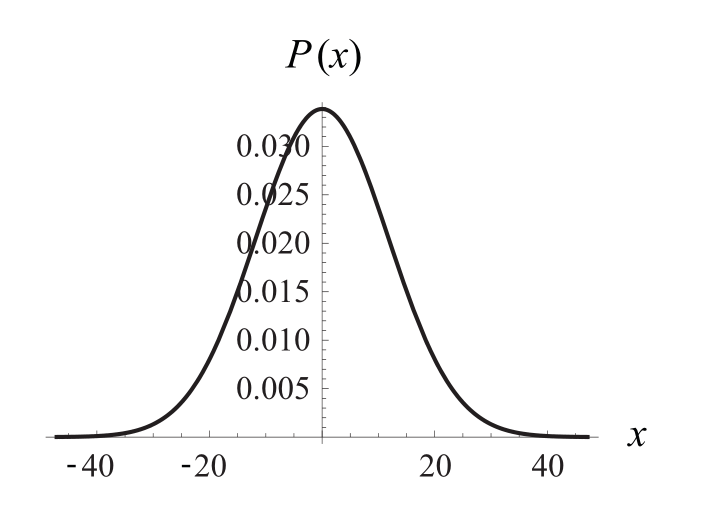
\includegraphics[width=0.6\linewidth]{figure5_15.png}}
    \caption*{\textbf{Figure 5.15}: The probability distribution for the number of 6's in 1000
    dice rolls, relative to the expected number, 167.}
\end{figure}

\vspace{1em}

\begin{proof}
    Both the dice and coin distributions are binomial distributions, so we'll approximate
    them as Gaussian distributions. A Gaussian distribution is uniquely identified by its
    mean and standard deviation, so two distributions are identical if they have these
    two attributes identical. Since we are interested by the distribution 
    for the number of Heads relative to the expected number, we don't care about the mean.
    Therefore, the standard deviation of the dice distribution must be the same as the one
    of the coin distribution. Knowing that the standard deviation for a Gaussian approximation
    of a binomial distribution is given by $\sqrt{np(1 - p)}$, and by considering fair coins/dice,
    we notice that the standard deviations of the distributions are equal for:
    \[
        \sqrt{1000 \cdot \frac{1}{6} \cdot \frac{5}{6}} = \sqrt{\frac{n}{4}} 
        \iff \frac{50\sqrt{2}}{6} = \frac{\sqrt{n}}{2}
        \iff 50\sqrt{2} = 3\sqrt{n} \iff n = \frac{5000}{9} \approx 556
    \] 

    Therefore, we need to flip 556 coins to obtain a very close Gaussian distribution to
    Fig. 5.15.
\end{proof}

\section*{5.5. Gambler's fallacy}
\addcontentsline{toc}{section}{5.5. Gambler's fallacy}
Assume that after 20 coin flips, you have obtained only five Heads. The
probability of this happening is small (about 1.5\%, since $\binom{20}{5} / 2^{20} = 0.0148$),
but not negligible. Since the law of large numbers says that the fraction of Heads approaches
50\% as the number of flips gets large, should you expect to see more Heads and Tails in
future flips?

\vspace{1em}

\begin{proof}
    Since coin flips are independent events, we can't make any assumption about future flips
    based on the already done 20 flips. Also, we can't assume anything based on the law of large
    numbers, since it assumes that the number of trials goes to infinity, so any unusual trends could
    occur at any time, and their effect will be diminished as the number of trials increases. 
\end{proof}

\section*{5.6. Finding the Gaussian}
\addcontentsline{toc}{section}{5.6. Finding the Gaussian}
What is the explicit form of the Gaussian function $f(x)$ that matches
up with the fourth histogram in Fig. 5.11? Assume that $n_t = 10$ is large
enough so that the Gaussian approximation does indeed hold.

\begin{figure}[H]
    \center{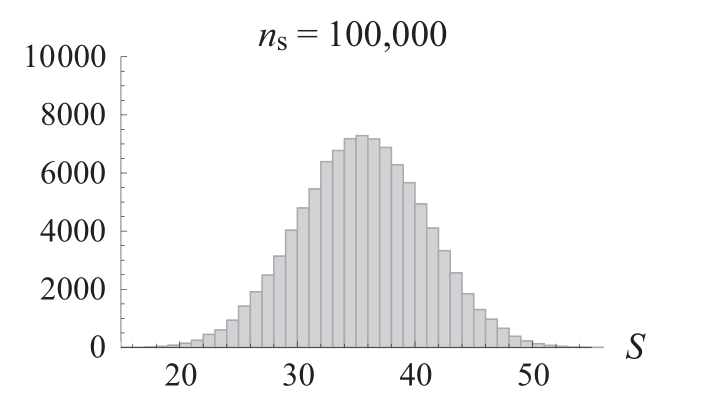
\includegraphics[width=0.6\linewidth]{figure5_15_histogram.png}}
    \caption*{\textbf{Figure 5.11}: Fourth Histogram}
\end{figure}

\vspace{1em}

\begin{proof}
    We assume that $n_t = 10$ is large enough so the Gaussian approximation holds.
    Let $X$ denote the outcome of a dice roll and let $Y$ represent the sum of 10 such outcomes,
    so $Y = X_1 + X_2 + \ldots X_{10}$, where the $X_i$s are distributed the same as $X$.
    One can easily show that $\sigma_X = 1.71$ and $\mu_X = 3.5$. The mean of $Y$ is easily
    obtained by using the linearity of expectation:
    \[
        \mu_Y = E[Y] = E\bigg[\sum_{i = 1}^{10}X_i\bigg] = 10E[X] = 10\mu_X = 35
    \] 

    The variance of $Y$ is computed by also using the fact that the $X_i$ variables
    are independent, so the expectation of their product can be split:
    \begin{align*}
        {\sigma_Y}^2 
        = E[Y^2] - {\mu_Y}^2 
        &= E\bigg[\bigg(\sum_{i = 1}^{10} X_i\bigg)^2\bigg] - 100\mu_X^2 
        = 10E[X^2] + 2\sum_{i = 1}^{10}\sum_{j = i + 1}^{10} E[X_i X_j] - 100\mu_X^2 \\
        &= 10E[X]^2 - 110\mu_X^2 + 10\mu_X^2 
        = 10E[X]^2 - 10\mu_X^2 = 10\sigma_X^2 \approx 29.24
    \end{align*}

    From the Central Limit Theorem, we know that $Y$ will be the Gaussian approximation 
    of the process described by the histogram. Therefore, since the probabilities
    represent the number of sums with a specific value (height of the columns), divided
    by the number of total sums ($n_s$), the Gaussian function associated to the histogram
    is given by the PDF of $Y$, scaled by $n_s$:
    \[
        f(x) = n_s G(y | \mu_Y, \sigma_Y^2) 
        = \frac{10^5}{29.24\sqrt{2\pi}} e^{-\frac{(y - 35)^2}{2\cdot 29.24^2}}
    \] 
\end{proof}

\section*{5.7. Standard deviations}
\addcontentsline{toc}{section}{5.7. Standard deviations}
Calculate the theoretically predicted standard deviations of the histograms in
Figs. 5.13 and 5.14, and check that your results are consistent with a visual
inspection of the histograms. You will need the result from Problem 4.3 for
Fig. 5.14.

\vspace{1em}

\begin{proof}
    We analyze the two figures separately:

    \vspace{1em}

    \textbf{Fig. 5.13} The histogram shows the result of taking $n_s = 10^5$ averages of
    $n_t = 100$ numbers chosen from the distribution in Fig. 5.12. Let $X$ be a
    random variable modeled by the distribution in Fig. 5.12. Then,
    \[
        P(X = 2) = 0.6 \hspace{2em} P(X = 3.1) = 0.1 \hspace{2em} P(X = 7) = 0.3
    \] 

    Therefore, the mean of $X$ is 
     \[
         \mu_X = E[X] = 2 \cdot 0.6 + 3.1 \cdot 0.1 + 7 \cdot 0.3 = 3.61
    \] 
    while the variance is given by
    \[
        \sigma_X^2 = E[(X - \mu)^2] = (2 - 3.61)^2 \cdot 0.6 + (3.1 - 3.61)^2 \cdot 0.1 + (7 - 3.61)^2 \cdot 0.3 
        \approx 5.26
    \] 

    Now, let $Y$ denote the average of $100$ numbers distributed like $X$ (denoted by $X_i$), so
    \[
        Y = \frac{1}{100}\sum_{i = 1}^{100} X_i
    \] 

    By using the linearity of expectation, the mean of $Y$ is
    \[
        \mu_Y = E[Y] = \frac{1}{100}E\bigg[\sum_{i = 1}^{100} X_i\bigg] 
        = \frac{1}{100}\sum_{i = 1}^{100} E[X_i] 
        = E[X] = \mu_X = 3.61
    \] 

    and the variance is given by:
    \[
        \text{Var}(Y) = \text{Var}\bigg(\frac{1}{100} \sum_{i = 1}^{100} X_i\bigg)
        = \frac{1}{10^4} \text{Var}\bigg(\sum_{i = 1}^{100} X_i\bigg)
        = \frac{1}{10^4} \sum_{i = 1}^{100} \text{Var}(X_i)
        = \frac{1}{100} \text{Var}(X) = 0.0526
    \]
    which gives the standard deviation:
    \[
        \sigma_Y \approx 0.23
    \] 

    \begin{figure}[H]%
        \centering
        \subfloat[\centering Histogram in Fig 5.13]{{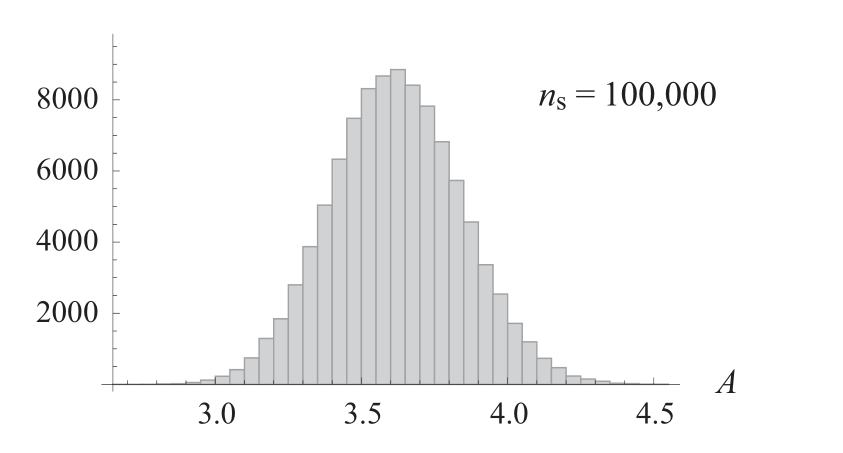
\includegraphics[width=0.49\linewidth]{5_7_fig513.png} }}%
        \qquad
        \subfloat[\centering Gaussian with $\mu = 3.61, \sigma = 0.23$, scaled by $10^5$]{{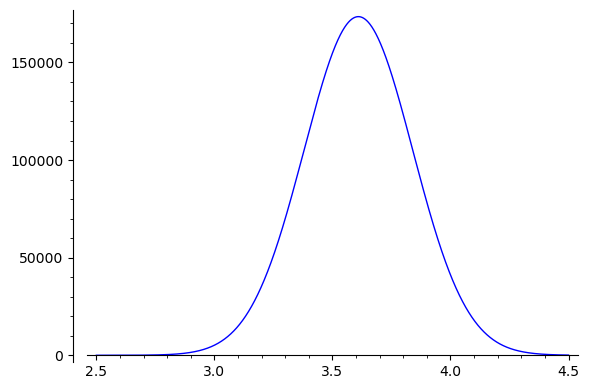
\includegraphics[width=0.44\linewidth]{5_7_gauss2.png} }}%
    \end{figure}

    \vspace{1em}

    \textbf{Fig. 5.14.} The histogram portrays the results of taking $n_s = 10^5$ averages
    of $n_t = 50$ numbers chosen from a uniform distribution (from 0 to 1). Let X be
    distributed by that uniform distribution. The mean of the uniform distribution 
    is just $\mu_X = 1/2$ and the variance is given by the result from Problem 4.3, i.e.
    $\sigma_X^2 = 1/12$. Now, let $Y$ denote the average of 50 numbers chosen from this
    distribution, so basically
    \[
        Y = \frac{1}{50} \sum_{i = 1}^{50} X_i
    \] 
    where the $X_i$ variables are distributed like $X$.
    If we assume that $n_t = 50$ is large enough for the Central Limit Theorem to apply,
    we find that $Y$ is modeled by a Gaussian distribution. Note that the 1/50 scaler
    does not change this, because a scaled Gaussian is still a Gaussian. Therefore, by
    using the linearity of expectation, we get the mean of $Y$:
    \[
        \mu_Y = E[Y] = \frac{1}{50}E\bigg[\sum_{i = 1}^{50} X_i\bigg] 
        = \frac{1}{50}\sum_{i = 1}^{50} E[X_i] 
        = E[X] = \mu_X = \frac{1}{2}
    \] 

    Similarly, by using the fact that the variance of a sum of random variables is equal
    to the sum of variances (for independent variables), we have that:
    \[
        \text{Var}(Y) = \text{Var}\bigg(\frac{1}{50} \sum_{i = 1}^{50} X_i\bigg)
        = \frac{1}{50^2} \text{Var}\bigg(\sum_{i = 1}^{50} X_i\bigg)
        = \frac{1}{50^2} \sum_{i = 1}^{50} \text{Var}(X_i)
        = \frac{1}{50} \text{Var}(X) = \frac{1}{600}
    \] 
    which gives the standard deviation
    \[
        \sigma_Y = \frac{1}{10\sqrt{6}}
    \] 

    We can confirm that this result is valid by comparing the plot of the corresponding Gaussian 
    function in the figure with the histogram and seeing that they are are very similar: 
    \begin{figure}[H]%
        \centering
        \subfloat[\centering Histogram in Fig 5.14]{{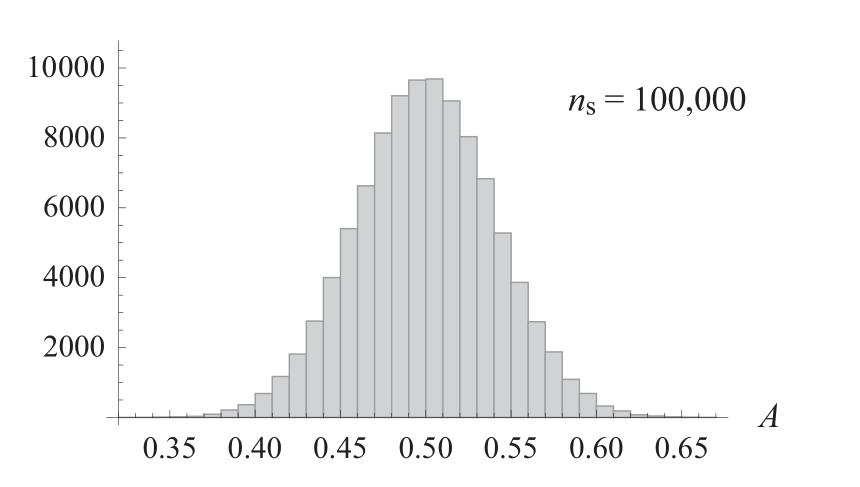
\includegraphics[width=0.49\linewidth]{5_7_fig514.png} }}%
        \qquad
        \subfloat[\centering Gaussian with $\mu = 1/2, \sigma = \frac{1}{10\sqrt{6}}$, scaled by $10^5$]{{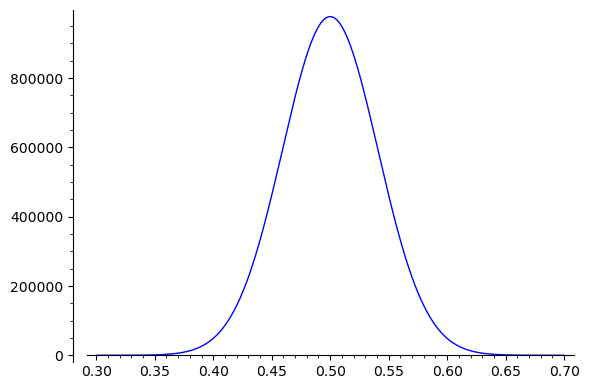
\includegraphics[width=0.44\linewidth]{5_7_gauss1.png} }}%
    \end{figure}
\end{proof}

    \chapter{Correlation and Regression}

\section*{6.1. Alternative forms of Cov(x, y) and $\bm{\widetilde{s}}$}
\addcontentsline{toc}{section}{6.1. Alternative forms of Cov(x, y) and $\widetilde{s}$}
\begin{enumerate}[(a)]
    \item Show that the Cov(x, y) defined in Eq. (6.11) can be written
        as  $\langle xy \rangle - \langle x \rangle \langle y \rangle$ 
        ($\langle x \rangle$ means the same thing as $\overline{x})$

    \item Show that the $\widetilde{s}^2$ defined in Eq. (3.60) can be
        written  as $\langle x^2 \rangle - \langle x \rangle^2$
\end{enumerate}

\vspace{1em}
\begin{proof}
    \hfill
    \begin{enumerate}[(a)]
        \item We start with Eq. (6.11) and use the average formula to obtain the desired result:
            \begin{align*}
                \text{Cov}(x, y) 
                = \frac{1}{n} \sum_{i = 1}^n (x_i - \langle x \rangle)(y_i - \langle y \rangle)
                &= \frac{1}{n} \sum_{i = 1}^n (x_iy_i - \langle x \rangle y_i - \langle y \rangle x_i +  
                    \langle x \rangle \langle y \rangle) \\
                &= \langle xy \rangle - 2 \langle x \rangle \langle y \rangle 
                    + \langle x \rangle \langle y \rangle
                = \langle xy \rangle - \langle x \rangle \langle y \rangle
            \end{align*}

        \item Similarly to (a), we start from Eq. (3.60) and find that:
            \begin{align*}
                \widetilde{s}^2 
                = \frac{1}{n} \sum_{i = 1}^n (x_i - \langle x \rangle)^2
                = \frac{1}{n} \sum_{i = 1}^n (x_i^2 - 2x_i \langle x \rangle + \langle x \rangle^2)
                = \langle x^2 \rangle - 2\langle x \rangle^2 + \langle x \rangle^2
                = \langle x^2 \rangle + \langle x \rangle^2 
            \end{align*}
    \end{enumerate}
\end{proof}

\section*{6.2. Rescaling X}
\addcontentsline{toc}{section}{6.2. Rescaling X}
Using Eq. (6.9), we showed in the third remark on page 287 that the
correlation coefficient $r$ doesn't change with a uniform scaling of
$X$ or $Y$. Demonstrate this again here by using the expression
for $r$ in Eq. (6.6).

\vspace{1em}

\begin{proof}
    Let $X' = aX$ and $Y' = bY$, where $a$ and $b$ are numerical values.
    Since $Y = mX + Z$, we notice the equivalence:
    \[
        bY = bmX + bZ \iff Y' = m'X' + cZ
    \] 
    where $m = bm/a$ and $c$ is a numerical value that we don't care about
    since the correlation coefficient $r$ does not depend on $Z$.
    From $(6.6)$ and the fact that $\text{Var}(aX) = a^2\text{Var}(X)$, we obtain:
     \[
         r' 
         = \frac{m'\sigma_{X'}}{\sigma_{Y'}} 
         = \frac{abm\sigma_{X}}{ab\sigma_{Y}}
         = \frac{m\sigma_X}{\sigma_Y} 
         = r
    \] 
    which proves once again that the correlation coefficient $r$ doesn't 
    change with a uniform scaling of $X$ or $Y$.
\end{proof}

\section*{6.3. Uncorrelated vs. independent}
\addcontentsline{toc}{section}{6.3. Uncorrelated vs. independent}
If two random variables $X$ and $Y$ are independent, are they necessarily
also uncorrelated? If they are uncorrelated, are they necessarily also independent?

\vspace{1em}

\begin{proof}
    \hfill
    \begin{enumerate}[(i)]
        \item Suppose $X$ and $Y$ are independent. We then have that $\text{Cov}(X, Y) = 0$, so,
            the correlation coefficient is given by (6.9):
            \[
                r = \frac{\text{Cov}(X, Y)}{\sigma_X\sigma_Y} = 0
            \] 
            As a result, if $X$ and $Y$ are independent, then they are also uncorrelated.

        \item We'll prove that correlation does not imply independence by giving a counterexample.
            Let $X$ be a discrete random variable with $P(X = 0) = P(X = 1) =$ 1/2 and let
            $Y = -X$. $X$ and $Y$ are independent and their covariance is given by
            \[
                \text{Cov}(X, Y) = E[XY] - \mu_X\mu_Y 
                = -E[X^2] + \frac{1}{4} 
                = -\bigg(\frac{1}{4} \cdot 1 + \frac{3}{4} \cdot 0\bigg) + \frac{1}{4}
                = 0
            \] 
            so, by (6.9), $r = 0$. Therefore, two random variables can be uncorrelated
            without being necessarily independent.
    \end{enumerate}
\end{proof}

\section*{6.4. Sum of two Gaussians (TO DO: PDF of sum)}
\addcontentsline{toc}{section}{6.4. Sum of two Gaussians}
Given two independent Gaussian distributions $X$ and $Y$ with
standard deviations $\sigma_X$ and $\sigma_Y$, show that the sum
$Z \equiv X + Y$ is a Gaussian distribution with standard
deviation $\sqrt{\sigma_X^2 + \sigma_Y^2}$. You may assume without
loss of generality that the means are zero.

\vspace{1em}

\begin{proof}
    We start by seeing that
    \[
        \mu_Z = E[Z] = E[X + Y] = \mu_X + \mu_Y
    \] 

    Now, by using the variance formula
    \[
        \sigma_Z^2 = E[Z^2] - \mu_Z^2 
        = E[(X+Y)^2] - \mu_Z^2
        = E[X^2 + 2XY + Y^2] - \mu_Z^2
    \] 

    By using the linearity of expectation and then the fact that $X$ and $Y$ are
    independent, our expression becomes:
     \[
         \sigma_Z^2 
         = E[X^2] + 2E[X]E[Y] + E[Y^2] - \mu_Z^2
         = E[X^2] + 2\mu_X\mu_Y + E[Y^2] - \mu_Z^2
    \] 

    We expand $\mu_Z^2$ and notice the expressions of $\sigma_X^2$ and $\sigma_Y^2$:
     \[
         \sigma_Z^2 = E[X^2] - \mu_X^2 + E[Y^2] - \mu_Y^2 = \sigma_X^2 + \sigma_Y^2
    \] 

    Finally, we take the square root of the variance to get the standard deviation:
    \[
        \sigma_Z = \sqrt{\sigma_X^2 + \sigma_Y^2}
    \] 
\end{proof}

\section*{6.5. Maximum $\bm{\rho(x, y)}$}
\addcontentsline{toc}{section}{6.5. Maximum $\rho(x, y)$}
For a given $y_0$, what value of $x$ maximizes the probability density
$\rho(x, y_0)$ in Eq. (6.34)?

\vspace{1em}

\begin{proof}
    The joint probability density $\rho(x, y_0)$ is given by
    \begin{equation*}\tag{6.34}
        \rho(x, y) = \frac{1}{2\pi\sigma_X\sigma_Y\sqrt{1 - r^2}} 
        \exp\bigg(-\frac{1}{2(1 - r^2)}\bigg(\frac{x^2}{\sigma_X^2} 
            + \frac{y_0^2}{\sigma_Y^2} - \frac{2rxy_0}{\sigma_X\sigma_Y}\bigg)\bigg)
    \end{equation*}

    Let
    \[
        \phi(x) 
        = \bigg(\frac{x^2}{\sigma_X^2} + \frac{y_0^2}{\sigma_Y^2} - \frac{2rxy_0}{\sigma_X\sigma_Y}\bigg) 
    \] 

    We notice that $x$ is used only in the second factor of the exponential, so
    $\rho(x, y_0)$ is maximised when $\phi(x)$ is minimised (there is a "-" sign in the exponential). We take the derivative of $\phi(x)$
    with respect to $x$ and  obtain
    \[
        \pdv{x} \phi(x) 
        = \pdv{x} \bigg(\frac{x^2}{\sigma_X^2} + \frac{y_0^2}{\sigma_Y^2} - \frac{2rxy_0}{\sigma_X\sigma_Y}\bigg) 
        = \frac{2x}{\sigma_X^2} - \frac{2ry_0}{\sigma_X\sigma_Y}
        = \frac{2x\sigma_Y - 2ry_0\sigma_X}{\sigma_X^2\sigma_Y}
    \] 

    If we equalize the derivative with 0, we obtain the critical point
    \[
        x_0 = ry_0 \frac{\sigma_X}{\sigma_Y}
    \] 

    Since the derivative is negative on the left of $x_0$ and positive on the right of $x_0$,
    we get that $x_0$ is the global minimum of $\phi(x)$. As a result, $x_0$ is the global maximum
    of $\rho(x, y_0)$.
\end{proof}

\section*{6.8. Alternate form of B}
\addcontentsline{toc}{section}{6.8. Alternate form of B}
Show that the second expression for $B$ in Eq. (6.49) equals
the first.

\vspace{1em}

\begin{proof}
    \begin{align*}\tag{6.49}
        \langle y \rangle - A \langle x \rangle 
        = \langle y \rangle - \langle x \rangle 
        \frac{\langle xy \rangle - \langle x \rangle \langle y \rangle}{\langle x^2 \rangle - \langle x \rangle^2}
        &= \frac{\langle y \rangle \langle x^2 \rangle - \langle y \rangle \langle x \rangle^2
            - \langle x \rangle \langle xy \rangle - \langle x \rangle^2 \langle y \rangle}
            {\langle x^2 \rangle - \langle x \rangle^2} \\
        &= \frac{\langle y \rangle \langle x^2 \rangle - \langle x \rangle \langle xy \rangle}
            {\langle x^2 \rangle - \langle x \rangle^2}
        = B
    \end{align*}
\end{proof}

\section*{6.9. Finding all the quantities}
\addcontentsline{toc}{section}{6.9. Finding all the quantities}
Given five ($X, Y$) points with values (2, 1), (3, 1), (3, 3),
(5, 4), (7, 6), calculate (with a calculator) all of the quantities
reffered to in the five steps listed on page 290. Also calculate
$B$ in Eq. (6.49), and make a rough plot of the five given points
along with the regression (least-squares) line.

\vspace{1em}

\begin{proof}
    \hfill
    \begin{enumerate}[1.]
        \item Compute the means $\overline{x}$ and $\overline{y}$ of the $x_i$ and 
             $y_i$ data points:
             \[
                 \overline{x} = \frac{2 + 3 + 3 + 5 + 7}{5} = 4
                 \hspace{2em}
                 \overline{y} = \frac{1 + 1 + 3 + 4 + 6}{5} = 3
             \] 

         \item Calculate the standard deviations $\widetilde{s_x}$ and $\widetilde{s_y}$ via 
             Eq. (3.60):
             \begin{align*}
                 \widetilde{s_x} = \sqrt{\frac{(2 - 4)^2 + (3 - 4)^2 + (3 - 4)^2 + (5 - 4)^2 + (7 - 4)^2}{5}} 
                    = \frac{4}{\sqrt{5}} \approx 1.79 \\
                \widetilde{s_y} = \sqrt{\frac{(1 - 3)^2 + (1 - 3)^2 + (3 - 3)^2 + (4 - 3)^2 + (6 - 3)^2}{5}}
                    = 3 \sqrt{\frac{2}{5}} \approx 1.9
             \end{align*}
            
        \item Calculate the covariance via Eq. (6.11):
            \begin{align*}
                \text{Cov}(x, y) 
                &= \frac{(2 - 4)(1 - 3) + (3 - 4)(1 - 3) + 
                    (3 - 4)(3 - 3) + (5 - 4)(4 - 3) + (7 - 4)(6 - 3)}{5} \\
                &= \frac{16}{5} = 3.2
            \end{align*}

        \item Calculate $r$ via Eq. (6.12):
            \[
                r = \frac{\text{Cov}(x, y)}{\widetilde{s_x}\widetilde{s_y}}
                = \frac{3.2}{1.79 \cdot 1.9} \approx 0.94
            \] 

        \item Calculate $m$ from Eq. (6.18), with the $\sigma$'s replaced with $\widetilde{s}$'s :
            \[
                m = \frac{r\widetilde{s_y}}{\widetilde{s_x}} 
                = \frac{0.94 \cdot 1.9}{1.79} \approx 1
            \] 
        \end{enumerate}
        \begin{figure}[H]     
        \center{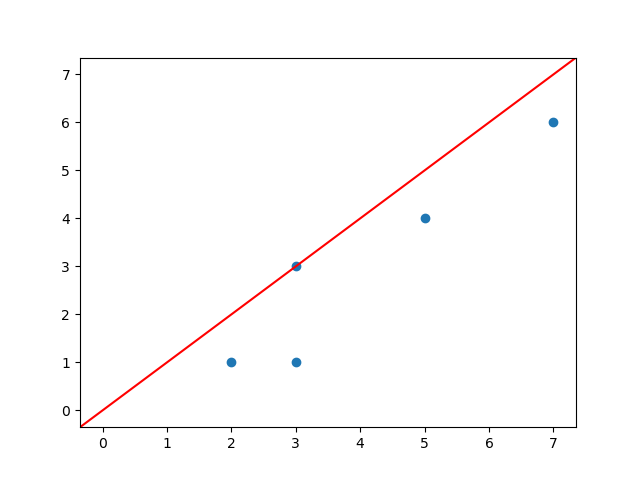
\includegraphics[width=0.50\linewidth]{figure_6_9.png}}
        \end{figure}
\end{proof}

\section*{6.10. Equal distances}
\addcontentsline{toc}{section}{6.10. Equal distances}
In Section 6.9. we defined the best-fit line as the line that minimizes
the sum of the squares of the vertical distance from the given point
to the line. Let's kick things down a dimension and look at the 1-D
case where we have $n$ values $x_i$ lying on the $x$ axis. We'll define
the "best-fit" point as the value of $x$ (call it $x_b$) that minimizes 
the sum of the squares of the distances from the  $n$ given $x_i$ points
to the $x_b$ point.

\begin{enumerate}[(a)]
    \item Show that $x_b$ is the mean of the $x_i$ values.
    
    \item Show that the sum of all the distances from $x_b$ to the
        points with $x_i > x_b$ equals the sum of all the distances
        from $x_b$ to the points with $x_i < x_b$.
\end{enumerate}

\vspace{1em}

\begin{proof}
    \hfill
    \begin{enumerate}[(a)]
        \item Let us define
            \[
                S \equiv \frac{1}{n} \sum_{i = 1}^n (x_i - x_b)^2
            \] 
            
        The value for $x_b$ for which $S$ is minimized can be found between the values
        for which the derivative of $S$ with respect to $x_b$ is 0. We have that:
        \[
            \pdv{x_b}S = \frac{1}{n} \sum_{i = 1}^n \pdv{x_b}(x_i^2 - 2x_i x_b + x_b^2) 
            = \frac{1}{n} \sum_{i = 1}^n (2x_b - 2x_i) = 2x_b - \frac{2}{n} \sum_{i = 1}^n x_i
            = 2x_b - 2\overline{x}
        \] 

        Therefore, $x_b = \overline{x}$ is a critical point for $S$. Since the slope
        of $S$ is positive and then negative around $x_b$, we obtain that $x_b = \overline{x}$
        is an absolute minimum point for $S$. 

    \item We can assume without loss of generality that the points are labeled such that
        for $i \leq M$, $x_i < x_b$ and for $i > M, x_i > x_b$. Hence, there are $M$ points
        that are less than $x_b$ and $(n - M)$ points that are greater than $x_b$. Our
        hypothesis becomes equivalent with the expression 
        \[
            \sum_{i = 1}^M (x_b - x_i) = \sum_{i = M + 1}^n (x_i - x_b)
        \] 
        We separate the $x_b$ terms from the sums and obtain that
        \[
            Mx_b - \sum_{i = 1}^M x_i = (M - n) x_b + \sum_{i = M + 1}^n x_i
        \] 

        If we isolate the $x_b$ from the sum terms, we have that
        \[
            nx_b = \sum_{i = 1}^{n} x_i
        \] 

        which with $x_b = \overline{x}$, the result that we proved at (a). Therefore,
        we proved the hypothesis.
    \end{enumerate}
\end{proof}

\section*{6.11. Equal distances again}
\addcontentsline{toc}{section}{6.11. Equal distances again}
Returning to 2-D, show that the sum of all the vertical distances from 
the least-squares line to the points above it equals the sum of all the vertical
distances from the line to the points below it. $\emph{Hint:}$ Consider an appropriate
partial derivative of the sum $S$ in Eq. (6.42).

\vspace{1em}

\begin{proof}
    The solution is similar to 6.10b. We assume without loss of generality that 
    the $n$ points are labeled such that for $i \leq M$,
    $y_i < Ax_i + B$ and  for $i > M, y_i > Ax_i + B$. Hence, there are $M$ 
    points that are under the least-squares line and $(n - M)$ above it. 
    Our hypothesis becomes equivalent with the expression
    \[
        \sum_{i = 1}^M (Ax_i + B - y_i) = \sum_{i = M + 1}^n (y_i - Ax_i + B)
    \] 
    We expand the sum to obtain that
    \[
        A \sum_{i = 1}^M x_i + BM - \sum_{i = 1}^M y_i 
        = \sum_{i = M + 1}^n y_i - A\sum_{i = M + 1}^n x_i + (n - M)B
    \] 
    We separate the $B$ terms from the rest of the expression and get that
    \[
        nB = \sum_{i = 1}^n y_i - A\sum_{i = 1}^n x_i 
    \] 
    which if we divide by $n$ and rewrite using the average operator, is equivalent with
    \begin{equation}\tag{6.49}
        B = \langle y \rangle - A \langle x \rangle
    \end{equation}
    which we know it's true. Therefore, we proved our hypothesis.
\end{proof}

\end{document}
